%% Copernicus Publications Manuscript Preparation Template for LaTeX Submissions
%% ---------------------------------
%% This template should be used for copernicus.cls
%% The class file and some style files are bundled in the Copernicus Latex Package which can be downloaded from the different journal webpages.
%% For further assistance please contact the Copernicus Publications at: publications@copernicus.org
%% http://publications.copernicus.org


%% Please use the following documentclass and Journal Abbreviations for Discussion Papers and Final Revised Papers.


%% 2-Column Papers and Discussion Papers
\documentclass[gmd, manuscript]{copernicus}



%% Journal Abbreviations (Please use the same for Discussion Papers and Final Revised Papers)

% Atmospheric Chemistry and Physics (acp)
% Advances in Geosciences (adgeo)
% Advances in Statistical Climatology, Meteorology and Oceanography (ascmo)
% Annales Geophysicae (angeo)
% ASTRA Proceedings (ap)
% Atmospheric Measurement Techniques (amt)
% Advances in Radio Science (ars)
% Advances in Science and Research (asr)
% Biogeosciences (bg)
% Climate of the Past (cp)
% Drinking Water Engineering and Science (dwes)
% Earth System Dynamics (esd)
% Earth Surface Dynamics (esurf)
% Earth System Science Data (essd)
% Fossil Record (fr)
% Geographica Helvetica (gh)
% Geoscientific Instrumentation, Methods and Data Systems (gi)
% Geoscientific Model Development (gmd)
% Geothermal Energy Science (gtes)
% Hydrology and Earth System Sciences (hess)
% History of Geo- and Space Sciences (hgss)
% Journal of Sensors and Sensor Systems (jsss)
% Mechanical Sciences (ms)
% Natural Hazards and Earth System Sciences (nhess)
% Nonlinear Processes in Geophysics (npg)
% Ocean Science (os)
% Primate Biology (pb)
% Scientific Drilling (sd)
% SOIL (soil)
% Solid Earth (se)
% The Cryosphere (tc)
% Web Ecology (we)



%% \usepackage commands included in the copernicus.cls:
%\usepackage[german, english]{babel}
%\usepackage{tabularx}
%\usepackage{cancel}
%\usepackage{multirow}
%\usepackage{supertabular}
%\usepackage{algorithmic}
%\usepackage{algorithm}
%\usepackage{float}
%\usepackage{subfig}
%\usepackage{rotating}

\usepackage{amsmath}
\usepackage{lineno}	% Dominik linenumbers
\usepackage{rotating}	% Dominik rotate table

\usepackage{marginnote} %Dominik for commments during drafting
\setlength{\marginparwidth}{35mm}


\begin{document}

%\linenumbers

\title{OMEN-SED 1.0: A new, numerically efficient sediment module for the coupling to Earth System Models}


% \Author[affil]{given_name}{surname}
\Author[1]{Dominik}{H\"ulse}
\Author[1]{Sandra}{Arndt}
\Author[2]{Stuart}{Daines}
\Author[1, 3]{Andy}{Ridgwell}

\affil[1]{School of Geographical Sciences, University of Bristol, Clifton, Bristol BS8 1SS, UK}
\affil[2]{Earth System Science, University of Exeter, North Park Road, Exeter EX4 4QE, UK}
\affil[3]{Department of Earth Sciences, University of California, Riverside, CA 92521, USA}

%% The [] brackets identify the author with the corresponding affiliation. 1, 2, 3, etc. should be inserted.



\runningtitle{OMEN-SED 1.0 - a sediment model for Earth System Models}

\runningauthor{H\"ulse et al.}

\correspondence{Sandra Arndt (s.arndt@bristol.ac.uk)}



\received{}
\pubdiscuss{} %% only important for two-stage journals
\revised{}
\accepted{}
\published{}

%% These dates will be inserted by Copernicus Publications during the typesetting process.


\firstpage{1}

\maketitle



\begin{abstract}
Here we describe the first version of the Organic Matter ENabled SEDiment model (OMEN-SED 1.0).
\end{abstract}



\introduction  %% \introduction[modified heading if necessary]
%>>>
\marginnote{\textbf{DH}: How to include comments.}[-1cm]%<<<
Marine surface sediments are key components in the Earth system. They host the largest carbon reservoir within the surficial Earth system, provide the only long term sink for atmospheric \chem{CO_2}, 
recycle nutrients and represent the most important climate archive. 
Biogeochemical processes in sediments depend on the water column and vice versa. Benthic processes are mainly donor controlled, as they are fuelled by the external supply of solid material 
(e.g. organic matter, calcium carbonate, opal) from the water column and are affected by overlying bottom water concentrations of solutes. At the same time, diagenesis in the sediments transforms the deposited 
material and returns the resulting products (e.g. nutrients, DIC) to the water column. 
This so-called benthic-pelagic coupling is essential for understanding the global carbon cycle and climate \citep[e.g.][]{archer_effect_1994, mackenzie_sediments_2005, ridgwell_role_2005}. 

\textcolor{red}{TODO:} Give examples when and why important (also in Paleo-context.

Degradation of organic matter (OM) in marine sediments fuels benthic biogeochemical processes and the resulting fluxes across the sediment-water interface are of considerable importance 
for many global biogeochemical cycles \citep{arndt_quantifying_2013}. Burial of OM represents an important connection between carbon stored in more climate-relevant reservoirs like the oceans, atmosphere, 
and the marine sediments and carbon that is sequestered for much longer, geological timescales in sedimentary rock or coal \citep{mackenzie_sediments_2005, burdige_preservation_2007}. 
Biological primary production of organic matter (\chem{CH_2O} in equation \ref{eq:photosynthesis}) and the reverse process of degradation can be written in a greatly simplified reaction as:
\begin{reaction}
\chem{CO_2}+\chem{H_2O} \rightleftharpoons \chem{CH_2O} + \chem{O_2}.\label{eq:photosynthesis}
\end{reaction}
On long timescales production of OM is generally greater than degradation which results in some organic matter being buried in marine sediments and oxygen accumulating in the atmosphere. 
Thus burial of OM leads to net oxygen input to, and \chem{CO_2} removal from, the atmosphere \citep{berner_phanerozoic_2004}. 
Therefore, globally quantifying the degradation of organic matter in marine sediments and related biogeochemical dynamics is important for understanding climate and the cycling of many chemical elements on various timescales.
Such studies and quantifications are possible through the application of idealised mathematical representations of diagenesis, or so-called diagenetic models \citep[e.g.][]{berner_early_1980, boudreau1997diagenetic}.
The number of research questions that can be addressed with diagenetic models is infinite and a plethora of different approaches have been developed, mainly following two distinct directions \citep{arndt_quantifying_2013}. 
First, state-of-the art diagenetic models simulating all of the essential coupled redox and equilibrium reactions within marine sediments that control carbon burial and benthic recycling fluxes 
(e.g. BRNS, \citeauthor{aguilera_knowledge-based_2005}, \citeyear{aguilera_knowledge-based_2005}; 
MEDIA, \citeauthor{meysman_reactive_2003}, \citeyear{meysman_reactive_2003}; OMEXDIA, \citeauthor{soetaert_model_1996}, \citeyear{soetaert_model_1996}). These ``complete'' models generally use a so-called multi-G approach, 
thus dividing the bulk organic carbon pool into a number of compound classes that are characterised by different degradabilities $k_i$. However, their global applicability is limited by the high computation cost of simulating 
all biogeochemical reactions. The second group of models is less sophisticated and comprehensive than the ``complete'' diagenetic models and is used for the coupling to global Earth System Models 
(e.g. DCESS, \citeauthor{shaffer_presentation_2008}, \citeyear{shaffer_presentation_2008}; HAMOCC, , \citeauthor{heinze_global_1999}, \citeyear{heinze_global_1999}; 
MEDUSA, \citeauthor{munhoven_glacialinterglacial_2007}, \citeyear{munhoven_glacialinterglacial_2007}). In particular, these models consider fewer biogeochemical reactions and apply the so-called 1G approach, 
thus just representing a single organic matter pool which is degraded at a constant rate. Obviously, such a simplification can neither account for the observed vast structural complexity in natural organic matter and its resulting 
different degradation rates nor for the decrease in OM degradability during diagenesis \citep{arndt_quantifying_2013}. 
A further problem of both approaches (and models in general) are model parameters which implicitly account for processes not explicitly described. These parameters are either derived through profile fitting for a specific site or 
follow different global relationships with a related, readily available sediment characteristic, such as water depth \citep{middelburg_empirical_1997} or sedimentation rate \citep{tromp_global_1995}. 
However, also these relationships are mostly based on simple fitting excercises to limited data sets and cannot replace a mechanistic representation of the underlying processes, especially when applying the model 
for different geological timescales. 

Even though there is potential to use more appropriate global sediment representations, in most current Earth System models sediment-water exchange of OM and chemical elements is generally treated in a very 
simplistic way \citep{soetaert_coupling_2000, huelse_biopump_models_2016}. 
Most Earth system Models of Intermediate Complexity (EMICs) for instance represent the sediment-water interface either as a reflective or a conservative/semi-reflective boundary \citep{huelse_biopump_models_2016}. 
Thus, all particulate material deposited on the seafloor is either instantaneously consumed (reflective boundary), or a fixed fraction is buried in the sediments (conservative/semi-reflective boundary). 
Both highly simplified approaches furthermore completely neglect the exchange of solute species through the sediment-water interface and, therefore, cannot resolve the complex benthic-pelagic coupling. 
However, due to their computational efficiency, both representations are often used in global biogeochemical models \citep[e.g.][]{najjar_impact_2007, ridgwell_marine_2007, goosse_description_2010}


\textcolor{red}{TODO:} Sandra review: large scale of published model parameters illustrates the complex nature of organic matter dynamics! Very difficult to find global relationships to relate model parameters 
to available environmental characteristics, such as water depth, deposition rate. Sentence about: even though there is some potential most ESM use the following:

See e.g. \citep{soetaert_coupling_2000, mackenzie_past_2004}.\\[2ex]

How are sediment resolved in Earth System models\\
See e.g. \citep{soetaert_coupling_2000}\\[2ex]
Problem with that: \\
The spatial variability in e.g. benthic particulate organic carbon (POC) mineralization kinetics throughout the ocean is currently unknown. This creates considerable 
uncertainties when diagenetic models are used to couple benthic and pelagic biogeochemical cycles in global models. \citep{kriest_numerical_2011} \\[2ex]

Alternative Model approaches, e.g. from coastal research\\[2ex]

Here, we present the OrganicMatter ENabled SEDiment model (OMEN-SED 1.0), a new, one-dimensional, numerically efficient reactive transport model (RTM) 
that describes OM cycling as well as the associated dynamics of the most important terminal electron acceptors (\chem{O_2,\ NO_3,\ SO_4,\ CH_4}), 
related reduced substances (\chem{NH_4,\ H_2S}) and macronutrients (\chem{PO_4}). %, DIC and Alkalinity.  
%for the biogeochemical dynamics of organic matter,  related chemical elements (\chem{O}, \chem{N}, \chem{S}, \chem{P}) and associated pore water quantities (ALK, DIC) in deep-sea sediments. 
OMEN-SEDs computational efficiency allows its coupling to Earth System Models and therefore the investigation of coupled global biogeochemical dynamics over geological timescales.
Also mention here presented as a 2G-Model, however OMEN-SED can easily be extended to a Multi-G approach. \\ [2ex]

See Van Cappellen and Wang (1996): ``Metal cycling in surface sediments: Modeling the interplay or transport and reaction'' for some good basic info! 

\section{Model Description}
The following section provides a detailed description of the new model. Table \ref{table:reactions_processes} summarizes the biogeochemical reaction network and 
a glossary of parameters along with their respective units is provided in Tables \ref{table:sed-charac_transport-parameters} and \ref{table:reaction_parameters}.

\subsection {General Model Approach} \label{subsec:GeneralModelApproach}
The calculation of benthic return/uptake and burial fluxes is based on the vertically resolved conservation equation for solid and dissolved species in porous media is given by 
\citep[e.g.][]{berner_early_1980, boudreau1997diagenetic}:

\begin{equation} 
\frac{\partial \xi C_i}{\partial t}=-\frac{\partial F}{\partial z}+\xi \sum_j R_i^j \label{eq:Eq_generaldiagenetic}
\end{equation}

where $C_i$ is the concentration of the biogeochemical species $i$, $\xi$ equals the porosity $\phi$ for solute species and $(1-\phi)$ for solid species, hence represents the partitioning of species $i$ 
into the solute and dissolved phase. The term $z$ is the sediment depth, $t$ denotes the time, $F$ summarises the transport fluxes and $\sum_j R_i^j$ represents the sum of production/consumption rates $j$ 
that affect species $i$. The reaction network has to account for the most important primary and secondary redox reactions, equilibrium reactions, mineral dissolution and precipitation, as well as adsorption 
and desorption processes that affect the explicitly resolved chemical species.\\
State-of-the-art reaction-transport models generally solve the ordinary differential equation (ODE) (eq. \ref{eq:Eq_generaldiagenetic}) numerically and thus allow to account for transient dynamics, 
depth-varying parameters or a high degree of coupling between different chemical species. Yet, numerical models are computational expensive, thus rendering their application in an Earth System Model framework prohibitive. 
An analytical solution of equation \eqref{eq:Eq_generaldiagenetic} provides an alternative and computational more efficient approach. Analytical models enjoyed great popularity in the early days of diagenetic modelling 
and computer technology due to their low computational demands. However, early analytical models were often very problem-specific and only considered one or two coupled species  \textcolor{red}{(e.g. Lehrman, Berner) ?? which pubs?}. 
Over the next decades, a number of more complex analytical models describing the coupled dynamics of ....were developed \citep[e.g.][]{billen1982modelling, goloway1982diagenetic, jahnke1982model}, 
before the boost in computing power enabled the development of fully-coupled, multi-species, numerical models \citep[e.g.][]{van1995metal, soetaert_model_1996}. 

\begin{figure}[htbp]
\begin{center}
	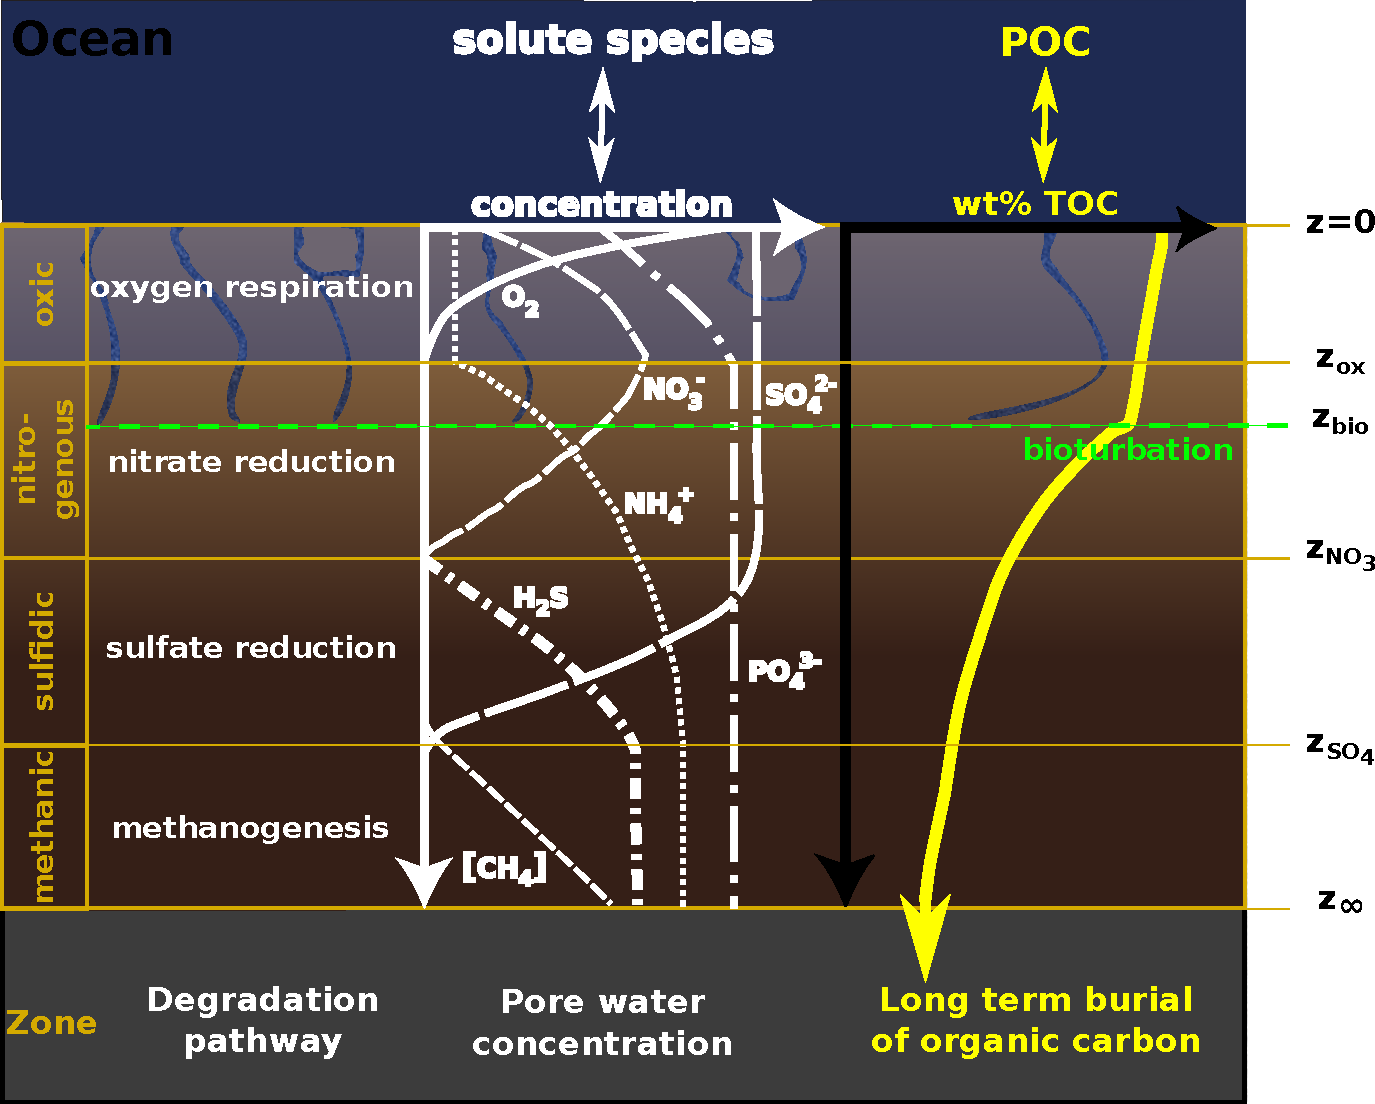
\includegraphics[width=0.8\textwidth]{figures/Sediment-model-with-profiles.pdf}
	\caption{Schematic of the different modelled species and layers in our sediment model. Here showing the case $z_{\mathrm{ox}} < z_{\mathrm{bio}} < z_{\chem{NO_3}} < z_{\chem{SO_4}}$.}
	\label{fig:Sediment_layers}
	\end{center}
\end{figure}

Finding an analytical solution to  Eq. (\ref{eq:Eq_generaldiagenetic}), especially when complex reaction networks are to be considered, is not straightforward and generally requires the assumption of steady state. 
In addition, the complexity of the reaction network can be reduced by dividing the sediment into distinct zones and accounting for the most pertinent biogeochemical processes 
within each zone, thus increasing the likelihood of finding an analytical solution to Eq. (\ref{eq:Eq_generaldiagenetic}). 

Therefore, OMEN-SED assumes that benthic dynamics can be represented by a series of steady-states. 
Because the Earth system model relevant variability in boundary conditions and fluxes is generally longer than the characteristic timescales of the reaction-transport processes, the sediment can be described by a 
series of pseudo steady-states. In addition, it divides the sediment into a bioturbated and a non-bioturbated zone defined by the constant bioturbation depth $z_{\mathrm{bio}}$ (see Fig. \ref{fig:Sediment_layers}). 
Furthermore, it accounts for the dynamic redox zonation of marine sediments by dividing the sediment into: 2) an oxic zone delineated by the oxygen 
penetration depth $z_{\mathrm{ox}}$, 3) a denitrification zone situated between $z_{\mathrm{ox}}$ and the nitrate penetration depth $z_{\chem{NO_3}}$, 4) 
a sulfate reduction zone situated between $z_{\chem{NO_3}}$ and the sulfate penetration depth $z_{\chem{SO_4}}$ and 5) a methanogenic zone situated below $z_{\chem{SO_4}}$ (Fig. \ref{fig:Sediment_layers}). 
All penetration depths are dynamically calculated by the model. 
Each zone is characterised by a set of diagenetic equations that encapsulate the most pertinent reaction and transport processes in this zone (see section \ref{subsec:Transport} and \ref{subsec:ReactionNetwork} 
for more details). 

OMEN calculates and feeds back to the Earth System model the fraction of POC preserved in the sediments and the sediment-water interface fluxes of the dissolved species $C_i$:
\begin{equation}
\mathrm{Flux\_SWI(C_i)} = \phi \cdot \left(D_i \frac{\partial C_i}{\partial z} + w C_i(0) \right)
\end{equation}
where $w$ is the deposition rate, $D_i$ is the diffusion coefficient and $C_i(0)$ the sediment-water concentration of species $i$. 

\subsection{Transport}\label{subsec:Transport}
The model accounts for both the advective, as well as the diffusive transport of dissolved and solid species, assuming that sediment compaction is negligible (i.e. $\frac{\partial \phi}{\partial z}=0$). 
The molecular diffusion of dissolved species is described via a species-specific apparent diffusion coefficient, $D_{\mathrm{mol},i}$. 
In addition, the activity of infaunal organisms in the bioturbated zone of the sediment ($z<z_{\mathrm{bio}}$) that causes random 
displacements of sediments and porewaters is simulated using a diffusive term (e.g. Boudreau,1986), with a constant bioturbation coefficient $D_{\mathrm{bio}}$ in the bioturbated zone. 
The pumping activity by burrow-dwelling animals and the resulting ventilation of tubes, the so-called bioirrigation, is encapsulated in a factor, $f_{ir}$ that enhances the molecular diffusion coefficient 
\citep[ hence, $D_{i,0}=D_{\mathrm{mol},i}\cdot f_{ir}$,][]{soetaert1996dynamic}. The flux divergence can thus be formulated as:
\begin{equation}
\frac{\partial F}{\partial z}=-\frac{\partial}{\partial z}\left( -\xi D_i \frac{\partial C_i}{\partial z} +\xi w C_i\right) \label{Eq_flux_divergence}
\end{equation}
where $D_i$ is the diffusion coefficient of species $i$ ($D_i=D_{i,0}+D_{\mathrm{bio}}=D_{\mathrm{mol},i}\cdot f_{ir}+D_{\mathrm{bio}}$ for dissolved species and $D_i=D_{\mathrm{bio}}$ for solid species) and $w$ is the deposition rate. 
The bioturbation coefficient $D_{\mathrm{bio}}$ is set to zero below $z_{\mathrm{bio}}$. In addition, infaunnal activity ceases ($D_{\mathrm{bio}}=0$) once bottom waters become anoxic ($\chem{O_2} < ???$ mol cm$^{-3}$ ). 
\textcolor{red}{check for good value + add if-query in code!!}

\subsection{Reaction Network}\label{subsec:ReactionNetwork}
Earth System models generally track the biogeochemical dynamics of organic and inorganic carbon, essential nutrients (nitrogen, phosphorus) and oxygen with the aim of investigating the evolution 
of the ocean's redox structure and carbonate system and its feedbacks on global climate. This general aim thus defines a minimum set of state variables and reaction processes that need to be resolved for an efficient 
representation of the benthic-pelagic coupling in Earth system models. A suitable sediment model must provide a robust quantification of organic (and inorganic) carbon burial fluxes, as well as 
the benthic return fluxes of growth-limiting nutrients, equilibrium invariant and reduced species, and oxygen uptake fluxes. 
As a consequence, the reaction network must account for the most important primary and secondary redox reactions, equilibrium reactions, 
mineral precipitation/dissolution and adsorption/desorption, resulting in a complex set of coupled reaction-transport equations. The following 
subsections provide a short discussion of the reaction processes included in the model and give an overview of the 
vertically resolved conservation equations and boundary conditions for solid and dissolved species in each layer. 
Table \ref{table:reactions_processes} provides a summary of the reactions and variables considered in the reaction network. Table \ref{table:Reaction_Network} summarises their reaction stoichiometry 
and Table \ref{table:ReactionOverview} provides an overview of their description in the model.

\begin{table}[tbp]
\caption{Reactions and variables implemented in the Reaction Network of OMEN-SED (1.0). The primary and secondary redox reactions are listed in the sequence they occur with increasing sediment depth.}
% title of Table
\centering
% used for centering table
\begin{tabular}{l l}
% centered columns (6 columns)
\hline\hline
%inserts double horizontal lines
 & Description\\
\hline
Primary redox reactions &  Degradation of organic matter via aerobic respiration, denitrification,\\
& sulfate reduction, methanogenesis (implicit)\\
Secondary redox reactions &  Oxidation of ammonium and sulfide by oxygen, anaerobic oxidation\\
& of methane by sulfate\\
Adsorption/Desorption & Ad-/Desorption of P on/from \chem{Fe(OH)_3}, \chem{NH_4} adsorption, \chem{PO_4} adsorption\\ %\textcolor{red}{Formation of Fe-bound P, reduction of Fe oxides (?correct here)},\\
Mineral precipitation & Formation of authigenic P \\
Variables & Organic matter, oxygen, nitrate, ammonium, sulfate, sulfide (hydrogen sulfide),\\
&  phosphate, Fe-bound P, DIC, ALK\\
\hline\hline
% inserts double horizontal lines
\end{tabular}
\label{table:reactions_processes}
% is used to refer this table in the text
\end{table}


\subsubsection{Organic matter}
In marine sediments, organic matter (OM) is degraded by heterotrophic activity coupled to the sequential utilisation of terminal electron acceptors (TEAs), typically in the order of \chem{O_2}, \chem{NO_3^-}, Mn(VI), Fe(III) and 
\chem{SO_4^{2-}} followed by methanogenesis and/or fermentation. Here, organic matter degradation is described via a multi-G model approach \citep[][and references therein]{arndt_quantifying_2013}, 
assuming that the bulk OM consists of a number of discrete compound classes $C_i$ characterised by specific degradation rate constants $k_i$. Such a multi-G approach allows for selective preservation of compound 
classes according to their reactivity, $k_i$ and, thus, accounts for the change in organic matter reactivity during burial. Each compound class is degraded according to first-order kinetics. 
The conservation equation for organic matter dynamics is thus given by:

\begin{equation}
 \frac{\partial C_i}{\partial t} = 0= D_{C_i} \frac{\partial^2C_i }{\partial z^2} - w\frac{\partial C_i }{\partial z} - k_i\cdot C_{i} \label{eq:ODE_OC}
\end{equation}
% where:
% \begin{align}
%  D_{C_i}&=D_{\mathrm{bio}} 	 &\text{if ($z\leq z_{\mathrm{bio}}$)}\\
%  D_{C_i}&=0            &\text{if ($z > z_{\mathrm{bio}}$)} 
% \end{align}
The analytical solution of Eq. \eqref{eq:ODE_OC} (see section \ref{sec:Solution} for details) requires the definition of a set of boundary conditions (Table \ref{Tab:BC_OM+O2}). 
The model assumes a known concentration/flux at the sediment-water interface and continuity across the bottom of the bioturbated zone, $z_{\mathrm{bio}}$.
\begin{table}[tbp]
\caption{Boundary conditions for organic matter and oxygen. For the boundaries we define:  $z^-_{\_\_} := \lim_{h\to0} (z_{\_\_}-h)$ and $z^+_{\_\_} := \lim_{h\to0} (z_{\_\_}+h)$.}
% title of Table
\centering
% used for centering table
\begin{tabular}{ |c| l| c l|}
\hline
\textbf{Boundary}& \textbf{Condition}& &\\
\hline
$z=0$& known concentration& 1)& $C_i(0)=C_{i0}$\\
$z=z_{\mathrm{bio}}$&continuity& 2)& $C_i(z_{\mathrm{bio}}^-)$=$C_i(z_{\mathrm{bio}}^+)$\\
               &&3)&$-D_{\mathrm{bio}}\cdot \frac{\partial C_i}{\partial z}|_{z_{\mathrm{bio}}^-}=0$\\
%Dom was               &&3) $D_{\mathrm{bio}}\cdot \frac{\partial C_i}{\partial z}|_{z_{\mathrm{bio}}^-}-w\cdot C_i(z_{\mathrm{bio}}^-)=-w\cdot C_i(z_{\mathrm{bio}}^+)$\\
\hline
$z=0$& known concentration& 1)&$\chem{O_2}(0)=O_{20}$\\
$z=z_{\mathrm{bio}}$&continuity& 2)&$ \chem{O_2}(z_{\mathrm{bio}}^-)$=$ \chem{O_2}(z_{\mathrm{bio}}^+)$\\
               &&3)&$-\left(D_{ \chem{O_2},0}+D_{\mathrm{bio}}\right )\cdot \frac{\partial  \chem{O_2}}{\partial z}|_{z_{\mathrm{bio}}^-}=-D_{ \chem{O_2},0} \cdot \frac{\partial  \chem{O_2}}{\partial z}|_{z_{\mathrm{bio}}^+}$\\
%Dom was               &&3) $\left(D_{\mathrm{bio}}+D_{mol, \chem{O_2}}\right )\cdot \frac{\partial  \chem{O_2}}{\partial z}|_{z_{\mathrm{bio}}^-}-w\cdot  \chem{O_2}(z_{\mathrm{bio}}^-)=D_{mol, \chem{O_2}} \cdot \frac{\partial  \chem{O_2}}{\partial z}|_{z_{\mathrm{bio}}^+}-w\cdot  \chem{O_2}(z_{\mathrm{bio}}^+)$\\
$z=z_{\mathrm{ox}}$&  \chem{O_2} consumption & 4)&\textbf{IF} $ (\chem{O_2}(z_\infty)> 0 )$\\
& ($z_{\mathrm{ox}} = z_\infty$) &&\quad $\frac{\partial  \chem{O_2}}{\partial z}|_{z_{\mathrm{ox}}}=0$ \\
& & &\textbf{ELSE} \\
& ($z_{\mathrm{ox}} < z_\infty$) & &\quad $  \chem{O_2}(z_{\mathrm{ox}})=0$  \quad and \quad $-D_{ \chem{O_2}} \cdot \frac{\partial  \chem{O_2}}{\partial z}|_{z_{\mathrm{ox}}}=F_{red}(z_\mathrm{ox})$\\
%$z=z_{\mathrm{ox}}$& & 5) $-D_{ \chem{O_2}} \cdot \frac{\partial  \chem{O_2}}{\partial z}|_{z_{\mathrm{ox}}}=F_{red, z_{\mathrm{ox}}}$\\   
&with flux from below &&$\quad F_{red}(z_\mathrm{ox})=\frac{1-\phi}{\phi} \cdot \int_{z_{\mathrm{ox}}}^{\infty}  \sum_i \left( 2\gamma_{\chem{NH_4}} \chem{NC_i} + \gamma_{\chem{H_2S}} \chem{SO_4C} \right) k_i C_i\ dz$ \\
% was from Sandra &with:&$F_{red,z_{\mathrm{ox}}}=\beta \cdot \int_{z_{\mathrm{ox}}}^{\inf}  \sum_i k_i\cdot C_i  dz  + 2\cdot \gamma \cdot \int_{z_{\mathrm{ox}}}^{\inf}  \sum_i k_i\cdot C_i  -  $ \\
\hline    
\end{tabular}
\label{Tab:BC_OM+O2}
% is used to refer this table in the text
\end{table}


\subsubsection{Oxygen}
In marine sediments, oxygen is consumed through the aerobic degradation of organic matter and a number of secondary redox reactions. 
In the oxic layer ($z<z_{ox}$), the model explicitly accounts for the aerobic degradation of OM, which consumes oxygen with a fixed O:C ratio (\chem{OC}, Tab. \ref{table:reaction_parameters}) 
and produces ammonium, which is partially nitrified to nitrate ($\gamma_\chem{NH_4}$).
%nitrification of parts of ammonium produced in the oxic layer of the sediment. 
%Oxygen serves as the most powerful terminal electron acceptor for the heterotrophic degradation of organic carbon. In addition, the oxidation of reduced species produced through microbial activity throughout the 
%sediment column further contributes to the consumption of oxygen. The model explicitly accounts for the consumption of oxygen by heterotrophic degradation and nitrification of ammonium in the oxic layer of the sediment. 
%The nitrification of 1 mol of ammonium in the oxic layer consumes 2 mol of oxygen. 
In addition, the oxygen consumption through the oxidation of reduced species (\chem{Fe^{2+}}, \chem{Mn^{2+}}, \chem{NH_4}, \chem{H_2S}) produced in the suboxic and anoxic layers of the sediment is implicitly taken into account 
through the flux boundary condition at the dynamic oxygen penetration depth $z_{\mathrm{ox}}$. This simplification can be justified as it has been shown that these secondary redox reactions mainly occur at the oxic/suboxic 
interface \citep{soetaert_model_1996}.  
The factor $\frac{1-\phi}{\phi}$ accounts for the volume conversion from the solid to the dissolved phase. 
%Oxygen is described in mol\,cm$^{-3}$ liquid and conversion from the solid phase of mineralized organic matter (expressed in mol\,cm$^{-3}$ bulk sediment) to consumption of dissolved oxygen (or later nutrients) introduce 
%a factor of $\frac{1-\phi}{\phi}$, where $\phi$ is the sediment porosity. 
Oxygen dynamics are thus described by:
\begin{align} 
 \frac{\partial \chem{O_2}}{\partial t} &= 0= D_{\chem{ \chem{O_2}}}\frac{\partial^2  \chem{O_2} }{\partial z^2} - w\frac{\partial  \chem{O_2}}{\partial z} - \frac{1-\phi}{\phi}\sum_i k_i \cdot [ OC + 2 \gamma_{\chem{NH_4}} \chem{NC_i} ]\cdot C_{i}(z) \label{eq:ODE_O2_1}
\end{align}
% where:
% \begin{align}
%  D_{ \chem{O_2}}&=D_{ \chem{O_2}, 0}+D_{\mathrm{bio}}  &\text{if ($z\leq z_{\mathrm{bio}}$)}\\
%  D_{ \chem{O_2}}&=D_{ \chem{O_2}, 0}                &\text{if ($z > z_{\mathrm{bio}}$)} 
% \end{align}  
The analytical solution of Eq. \eqref{eq:ODE_O2_1} (see section \ref{sec:Solution}) requires the definition of boundary conditions (Table \ref{Tab:BC_OM+O2}). 
The model assumes a known bottom water concentration and the complete consumption of oxygen at the oxygen penetration depth (or zero flux if $z_{\mathrm{ox}}=z_\infty$). 
It considers equal oxygen concentration and diffusive flux above ($z_{\mathrm{bio}}^-$) and 
below ($z_{\mathrm{bio}}^+$) the bioturbation boundary. In addition, the model imposes a flux of reduced species through the bottom of the oxic zone that is calculated as the reduced substances produced through anoxic mineralization 
of organic matter below $z_{\mathrm{ox}}$. Thus, assuming that fractions ($\gamma_{\chem{NH_4}}$ and $\delta$) of these reduced species are oxidised at the oxic/suboxic interface.
%\textcolor{red}{does not $\gamma_{\chem{NH_4}}, \delta$ account for part which is not oxidised?}
% was Sandra: In addition, it imposes a flux of reduce species through the bottom of the oxic zone that is calculated by integrating organic matter degradation rate and, thus, 
%assumes a complete oxidation of these species at the oxic/suboxic interface:   
\subsubsection{Nitrate and Ammonium}
%Nitrate and ammonium are described in $mol\ cm^{-3}$ liquid and a factor of $\frac{1-\phi}{\phi}$ is introduced to account for the conversion from mineralization rates to production of dissolved species. 
%To model nutrient dynamics the sediment is partitioned into two geochemical layers (oxic and suboxic)
To model nitrate and ammonium dynamics the sediment is partitioned into two geochemical layers (oxic and suboxic), where different equations describe the biogeochemical processes. 
Above the oxygen penetration depth organic matter mineralization produces ammonium, which is partly nitrified to nitrate (the fraction $\gamma_{\chem{NH_4}}$). 
In the suboxic zone ($z>z_{\mathrm{ox}}$), oxygen concentration is zero and nitrate serves as the electron acceptor to respire organic matter, thus nitrate is consumed by denitrification and ammonium is produced. Below the nitrate 
penetration depth $z_{\chem{NO_3}}$, ammonium is still produced through OM mineralization. Therefore the diagenetic equations for nitrate and ammonium are given by:
\begin{align}
\intertext{1. Layer ($z \leq z_{\mathrm{ox}}$)}
 \frac{\partial NO_3^I}{\partial t} &= 0 = D_{NO_3} \frac{\partial^2NO_3^I }{\partial z^2} - w\frac{\partial NO_3^I }{\partial z} + \gamma_{\chem{NH_4}} \frac{1-\phi}{\phi} \cdot \sum_i \chem{NC_i} \cdot k_i \cdot C_{i}(z)\label{eq:NO3_ODE1_L1}\\ %\qquad &\text{1. Layer ($z\leq z_{\mathrm{ox}}$)}\\
 \frac{\partial \chem{NH_4}^I}{\partial t} &= 0 = \frac{D_{\chem{NH_4}}}{1+K_\chem{NH_4}} \frac{\partial^2\chem{NH_4}^I }{\partial z^2} - w\frac{\partial \chem{NH_4}^I }{\partial z} + \frac{1-\gamma_{\chem{NH_4}}}{1+K_\chem{NH_4}}\cdot \frac{1-\phi}{\phi} \cdot \sum_i \chem{NC_i} \cdot k_i \cdot C_{i}(z)\label{eq:NH4_ODE1_L1}\\
 \intertext{2. Layer ($z_{\mathrm{ox}} < z \leq z_{\chem{NO_3}}$)} 
\frac{\partial NO_3^{II}}{\partial t} &= 0 = D_{NO_3} \frac{\partial^2NO_3^{II} }{\partial z^2} - w\frac{\partial NO_3^{II} }{\partial z} - \frac{1-\phi}{\phi} NO_3C \cdot \sum_i k_i \cdot C_{i}(z) \label{eq:NO3_ODE1_L2}\\
\frac{\partial \chem{NH_4}^{II}}{\partial t} &= 0 = \frac{D_{\chem{NH_4}}}{1+K_\chem{NH_4}} \frac{\partial^2\chem{NH_4}^{II} }{\partial z^2} - w\frac{\partial \chem{NH_4}^{II} }{\partial z} \label{eq:NH4_ODE1_L2}
 \intertext{3. Layer ($z_{\chem{NO_3}} < z \leq z_\infty$)} 
\frac{\partial \chem{NH_4}^{III}}{\partial t} &= 0 = \frac{D_{\chem{NH_4}}}{1+K_\chem{NH_4}} \frac{\partial^2\chem{NH_4}^{III} }{\partial z^2} - w\frac{\partial \chem{NH_4}^{III} }{\partial z} + \frac{1}{1+K_\chem{NH_4}}\cdot\frac{1-\phi}{\phi} \cdot \sum_i \chem{NC_i} \cdot k_i \cdot C_{i}(z)\label{eq:NH4_ODE1_L2}
\end{align}
% where
% \begin{align}
%  D_{i}&=D_{i, 0}+D_{\mathrm{bio}} &\text{if ($z\leq z_{\mathrm{bio}}$)}\\
%  D_{i}&=D_{i, 0}                &\text{if ($z > z_{\mathrm{bio}}$)} 
% \end{align} 
% and $i \in \{$NO$_3$, NH$_4\}$. 
The boundary conditions to solve Equations \ref{eq:NO3_ODE1_L1} - \ref{eq:NH4_ODE1_L2} are summarized in Table \ref{Tab:BC_NO3+NH4}. The model assumes known bottom water concentrations 
for both species, the complete consumption of nitrate at the nitrate penetration depth (or zero flux if $z_{\chem{NO_3}}=z_\infty$) and no change in ammonium flux at $z_\infty$. It considers equal concentrations and diffusive fluxes 
at $z_{\mathrm{bio}}$ and $z_{\mathrm{ox}}$.  In addition, the re-oxidation of upward-diffusing reduced ammonium is considered in the oxic-suboxic boundary condition for nitrate and ammonium. 

\begin{table}[tbp]
\caption{Boundary conditions for nitrate and ammonium.}
% title of Table
\centering
% used for centering table
\begin{tabular}{ |c| c| c l|}
\hline
\textbf{Boundary}& \textbf{Condition}& &\\
\hline
$z=0$& known concentration& 1)& $NO_3(0)=NO_{30}$  \\
$z=z_{\mathrm{bio}}$&continuity& 2)& $NO_3(z_{\mathrm{bio}}^-)$=$NO_3(z_{\mathrm{bio}}^+)$\\
               && 3)& $-\left(D_{NO_3,0}+D_{\mathrm{bio}}\right )\cdot \frac{\partial NO_3}{\partial z}|_{z_{\mathrm{bio}}^-}=-D_{NO_3,0} \cdot \frac{\partial NO_3}{\partial z}|_{z_{\mathrm{bio}}^+}$\\
$z=z_{\mathrm{ox}}$& continuity& 4)& $NO_3(z_{\mathrm{ox}}^-)$=$NO_3(z_{\mathrm{ox}}^+)$\\
               && 5)& $-D_{NO_3} \cdot \frac{\partial NO_3}{\partial z}|_{z_{\mathrm{ox}}^-} + \gamma_{\chem{NH_4}}\cdot F_{\chem{NH_4}}(z_{\mathrm{ox}})=-D_{NO_3} \cdot \frac{\partial NO_3}{\partial z}|_{z_{\mathrm{ox}}^+}$\\
&where: & &$ F_{\chem{NH_4}}(z_{\mathrm{ox}})=\frac{1}{1+K_\chem{NH_4}}\cdot \frac{1-\phi}{\phi} \cdot \int_{z_{\chem{NO_3}}}^{\infty}  \sum_i k_i \cdot \chem{NC_i} \cdot C_i\ dz$ \\          
$z=z_{\chem{NO_3}}$& \chem{NO_3} consumption & 6) & \textbf{IF} $ (\chem{NO_3}(z_\infty)> 0 )$\\
& ($z_{\chem{NO_3}} = z_\infty$) & & \quad $\frac{\partial NO_3}{\partial z}|_{z_{\chem{NO_3}}}=0$\\
& & &\textbf{ELSE} \\
& ($z_{\chem{NO_3}} < z_\infty$) & &\quad $NO_3(z_{\chem{NO_3}})=0$ \\
% was from Sandra &with:&$F_{red,z_{\mathrm{ox}}}=\beta \cdot \int_{z_{\mathrm{ox}}}^{\inf}  \sum_i k_i\cdot C_i  dz  + 2\cdot \gamma \cdot \int_{z_{\mathrm{ox}}}^{\inf}  \sum_i k_i\cdot C_i  -  $ \\
\hline
$z=0$& known concentration& 1)& $\chem{NH_4}(0)= \chem{NH_{40}}$  \\
$z=z_{\mathrm{bio}}$&continuity& 2)& $\chem{NH_4}(z_{\mathrm{bio}}^-)$=$\chem{NH_4}(z_{\mathrm{bio}}^+)$\\
               && 3)& $-\frac{D_{\chem{NH_4},0}+D_{\mathrm{bio}}}{1+K_\chem{NH_4}}\cdot \frac{\partial \chem{NH_4}}{\partial z}|_{z_{\mathrm{bio}}^-}=-\frac{D_{\chem{NH_4},0}}{1+K_\chem{NH_4}} \cdot \frac{\partial \chem{NH_4}}{\partial z}|_{z_{\mathrm{bio}}^+}$\\
$z=z_{\mathrm{ox}}$& continuity& 4)& $\chem{NH_4}(z_{\mathrm{ox}}^-)$=$\chem{NH_4}(z_{\mathrm{ox}}^+)$\\
  & & 5)& $-\frac{D_{\chem{NH_4}}}{1+K_\chem{NH_4}} \cdot \frac{\partial \chem{NH_4}}{\partial z}|_{z_{\mathrm{ox}}^-} -\gamma_{\chem{NH_4}}\cdot F_{\chem{NH_4}}(z_{\mathrm{ox}})=-\frac{D_{\chem{NH_4}}}{1+K_\chem{NH_4}} \cdot \frac{\partial \chem{NH_4}}{\partial z}|_{z_{\mathrm{ox}}^+}$\\
&where: & & $F_{\chem{NH_4}}(z_{\mathrm{ox}})=\frac{1}{1+K_\chem{NH_4}}\cdot \frac{1-\phi}{\phi} \cdot \int_{z_{\chem{NO_3}}}^{\infty}  \sum_i k_i \cdot \chem{NC_i} \cdot C_i\ dz$ \\          
$z=z_{\chem{NO_3}}$&continuity& 6)& $\chem{NH_4}(z_{\chem{NO_3}}^-)$=$\chem{NH_4}(z_{\chem{NO_3}}^+)$\\
               & flux & 7)& $-\frac{D_{\chem{NH_4}}}{1+K_\chem{NH_4}}\cdot \frac{\partial \chem{NH_4}}{\partial z}|_{z_{\chem{NO_3}}^-}=-\frac{D_{\chem{NH_4}}}{1+K_\chem{NH_4}} \cdot \frac{\partial \chem{NH_4}}{\partial z}|_{z_{\chem{NO_3}}^+}$\\
$z=z_{\infty}$& zero \chem{NH_4} flux & 8)& $\frac{\partial \chem{NH_4}}{\partial z}|_{z_\infty}=0$\\
\hline    
\end{tabular}
\label{Tab:BC_NO3+NH4}
\end{table}
\subsubsection{Sulfate and Sulfide}
When nitrate is depleted, sulfate reduction is the pathway to mineralize organic matter, thus consuming sulfate (SO$_4$) and producing hydrogen sulfide (H$_2$S) until the sulfate penetration depth ($z_{\chem{\chem{SO_4}}}$). 
Sulfate and sulfide dynamics are thus described by:
\begin{align}
\intertext{1. Layer ($z \leq z_{\chem{NO_3}}$)}
 \frac{\partial \chem{SO_4}^I}{\partial t} &= 0 = D_{\chem{SO_4}} \frac{\partial^2\chem{SO_4}^I }{\partial z^2} - w\frac{\partial \chem{SO_4}^I }{\partial z} \label{eq:SO4_ODE1_L1}\\ %\qquad &\text{1. Layer ($z\leq z_{\mathrm{ox}}$)}\\
 \frac{\partial \chem{H_2S}^I}{\partial t} &= 0 = D_{\chem{H_2S}} \frac{\partial^2\chem{H_2S}^I }{\partial z^2} - w\frac{\partial \chem{H_2S}^I }{\partial z}\label{eq:H2S_ODE1_L1}\\
 \intertext{2. Layer ($z_{\chem{NO_3}} < z \leq z_{\chem{SO_4}}$)} 
\frac{\partial \chem{SO_4}^{II}}{\partial t} &= 0 = D_{\chem{SO_4}} \frac{\partial^2\chem{SO_4}^{II} }{\partial z^2} - w\frac{\partial \chem{SO_4}^{II} }{\partial z} - \frac{1-\phi}{\phi} \cdot \sum_i \chem{SO_4C} \cdot k_i \cdot C_{i}(z) \label{eq:SO4_ODE1_L2}\\
\frac{\partial \chem{H_2S}^{II}}{\partial t} &= 0 = D_{\chem{H_2S}} \frac{\partial^2\chem{H_2S}^{II} }{\partial z^2} - w\frac{\partial \chem{H_2S}^{II} }{\partial z} + \frac{1-\phi}{\phi} \cdot \sum_i \chem{SO_4C}  \cdot k_i \cdot C_{i}(z)\label{eq:H2S_ODE1_L2}
 \intertext{3. Layer ($z_{\chem{SO_4}} < z \leq z_{\infty}$)} 
\frac{\partial \chem{H_2S}^{III}}{\partial t} &= 0 = D_{\chem{H_2S}} \frac{\partial^2\chem{H_2S}^{III} }{\partial z^2} - w\frac{\partial \chem{H_2S}^{III} }{\partial z}\label{eq:H2S_ODE1_L3}
\end{align}
% where
% \begin{align}
%  D_{i}&=D_{i, 0}+D_{\mathrm{bio}} &\text{if ($z\leq z_{\mathrm{bio}}$)}\\
%  D_{i}&=D_{i, 0}                &\text{if ($z > z_{\mathrm{bio}}$)} 
% \end{align} 
% and $i \in \{$SO$_4$, H$_2$S$\}$. 
To solve equations \ref{eq:SO4_ODE1_L1} - \ref{eq:H2S_ODE1_L3} the model assumes known concentrations at the sediment-water interface and continuity 
across the bioturbation depth and the nitrate penetration depth (see Table \ref{Tab:BC_SO4+H2S}). 
The re-oxidation of reduced \chem{H_2S} to \chem{SO_4} is considered in the 
oxic-suboxic boundary condition for both species, here including the methanic zone, as \chem{H_2S} is also produced during anaerobic oxidation of methane (AOM). 
Furthermore, sulfate is used at $z_{\chem{SO_4}}$ to oxidize methane from below and thus producing \chem{H_2S}. 
In case $z_{\chem{SO_4}}<z_\infty$, sulfate concentration is zero at $z_{\chem{SO_4}}$ and its diffusive flux must equal the amount of methane produced below; or, in case $z_{\chem{SO_4}}=z_\infty$, 
a zero flux condition for sulfate is considered. At lower boundary ($z_\infty$) zero flux of \chem{H_2S} is considered. 
%Additionally H$_2$S is produced by AOM which is considered in the flux boundary condition at $z_{\chem{SO_4}}$. 
\textcolor{red}{correct??}\\

\begin{table}[tbp]
\caption{Boundary conditions for sulfate and sulfide.}
% title of Table
\centering
% used for centering table
\begin{tabular}{ |c| c| c l|}
\hline
\textbf{Boundary}& \textbf{Condition}&&\\
\hline
$z=0$& known concentration& 1)& \chem{SO_4}(0)=\chem{SO_{40}}  \\
$z=z_{\mathrm{bio}}$&continuity& 2)& $\chem{SO_4}(z_{\mathrm{bio}}^-)$=$\chem{SO_4}(z_{\mathrm{bio}}^+)$\\
               & flux & 3)& $-\left(D_{\chem{SO_4},0}+D_{\mathrm{bio}}\right )\cdot \frac{\partial \chem{SO_4}}{\partial z}|_{z_{\mathrm{bio}}^-}=-D_{\chem{SO_4},0} \cdot \frac{\partial \chem{SO_4}}{\partial z}|_{z_{\mathrm{bio}}^+}$\\
$z=z_{\mathrm{ox}}$& continuity& 4)& $\chem{SO_4}(z_{\mathrm{ox}}^-)$=$\chem{SO_4}(z_{\mathrm{ox}}^+)$\\
               & flux & 5)& $-D_{\chem{SO_4}} \cdot \frac{\partial \chem{SO_4}}{\partial z}|_{z_{\mathrm{ox}}^-} + \gamma_{\chem{H_2S}}\cdot F_{\chem{H_2S}}(z_{\mathrm{ox}})=-D_{\chem{SO_4}} \cdot \frac{\partial \chem{SO_4}}{\partial z}|_{z_{\mathrm{ox}}^+}$\\
&where:& &$\quad F_{\chem{H_2S}}(z_{\mathrm{ox}})=\frac{1-\phi}{\phi} \cdot \left( \int_{z_{\chem{NO_3}}}^{\chem{SO_4}}  \sum_i \chem{SO_4C} \cdot k_i \cdot C_i\ dz + \gamma_\chem{CH_4}\cdot \int_{z_{\chem{SO_4}}}^{\infty}  \sum_i \chem{MC} \cdot k_i \cdot C_i\ dz \right)$\\          
$z=z_{\chem{NO_3}}$&continuity& 6)& $\chem{SO_4}(z_{\chem{NO_3}}^-)$=$\chem{SO_4}(z_{\chem{NO_3}}^+)$\\
               & flux & 7)& $-D_{\chem{SO_4}}\cdot \frac{\partial \chem{SO_4}}{\partial z}|_{z_{\chem{NO_3}}^-}=-D_{\chem{SO_4}} \cdot \frac{\partial \chem{SO_4}}{\partial z}|_{z_{\chem{NO_3}}^+}$\\
$z=z_{\chem{SO_4}}$& SO$_4$ consumption & 8)&  \textbf{IF} $ (\chem{SO_4}(z_\infty)> 0 )$\\
& ($z_{\chem{SO_4}} = z_\infty$) && \quad $\frac{\partial SO_4}{\partial z}|_{z_{\chem{SO_4}}}=0$\\
& & &\textbf{ELSE} \\
& ($z_{\chem{SO_4}} < z_\infty$) && \quad $\chem{SO_4}(z_{\chem{SO_4}})=0$ \quad and \quad $-D_{\chem{SO_4}} \cdot \frac{\partial \chem{SO_4}}{\partial z}|_{z_{\chem{SO_4}}}= \gamma_\chem{CH_4} \cdot F_{\chem{CH_4}}(z_{\chem{SO_4}})$\\%\quad \textcolor{red}{or/and (???)} \quad $\frac{\partial \chem{SO_4}}{\partial z}|_{z_{\chem{SO_4}}}= 0$\\   
&with flux from below:& &$ \quad F_{\chem{CH_4}}(z_{\chem{SO_4}})=\frac{1-\phi}{\phi} \cdot \int_{z_{\chem{SO_4}}}^{\infty}  \sum_i \chem{MC} \cdot k_i \cdot C_i\ dz$ \\
% was from Sandra &with:&$F_{red,z_{\mathrm{ox}}}=\beta \cdot \int_{z_{\mathrm{ox}}}^{\inf}  \sum_i k_i\cdot C_i  dz  + 2\cdot \gamma \cdot \int_{z_{\mathrm{ox}}}^{\inf}  \sum_i k_i\cdot C_i  -  $ \\
\hline
$z=0$& known concentration& 1)& $\chem{H_2S}(0)=\chem{H_2S}_{0}$  \\
$z=z_{\mathrm{bio}}$&continuity& 2)& $\chem{H_2S}(z_{\mathrm{bio}}^-)$=$\chem{H_2S}(z_{\mathrm{bio}}^+)$\\
               & flux & 3)& $-\left(D_{\chem{H_2S},0}+D_{\mathrm{bio}}\right )\cdot \frac{\partial \chem{H_2S}}{\partial z}|_{z_{\mathrm{bio}}^-}=-D_{\chem{H_2S},0} \cdot \frac{\partial \chem{H_2S}}{\partial z}|_{z_{\mathrm{bio}}^+}$\\
$z=z_{\mathrm{ox}}$& continuity& 4)& $\chem{H_2S}(z_{\mathrm{ox}}^-)$=$\chem{H_2S}(z_{\mathrm{ox}}^+)$\\
               & flux & 5)& $-D_{\chem{H_2S}} \cdot \frac{\partial \chem{H_2S}}{\partial z}|_{z_{\mathrm{ox}}^-} - \gamma_\chem{H_2S}  F_{\chem{H_2S}}(z_{\mathrm{ox}})=-D_{\chem{H_2S}} \cdot \frac{\partial \chem{H_2S}}{\partial z}|_{z_{\mathrm{ox}}^+}$\\
&where: & &$\quad F_{\chem{H_2S}}(z_{\mathrm{ox}})=\frac{1-\phi}{\phi} \cdot \left( \int_{z_{\chem{NO_3}}}^{\chem{SO_4}}  \sum_i \chem{SO_4C} \cdot k_i \cdot C_i\ dz + \gamma_\chem{CH_4}\cdot \int_{z_{\chem{SO_4}}}^{\infty}  \sum_i \chem{MC} \cdot k_i \cdot C_i\ dz \right)$\\            
$z=z_{\chem{NO_3}}$&continuity& 6)& $\chem{H_2S}(z_{\chem{NO_3}}^-)$=$\chem{H_2S}(z_{\chem{NO_3}}^+)$\\
               & flux & 7)& $-D_{\chem{H_2S}}\cdot \frac{\partial \chem{H_2S}}{\partial z}|_{z_{\chem{NO_3}}^-}=-D_{\chem{H_2S}} \cdot \frac{\partial \chem{H_2S}}{\partial z}|_{z_{\chem{NO_3}}^+}$\\
$z=z_{\chem{SO_4}}$& continuity & 8)& $\chem{H_2S}(z_{\chem{SO_4}}^-)$=$\chem{H_2S}(z_{\chem{SO_4}}^+)$\\ %$\frac{\partial \chem{H_2S}}{\partial z}|_{z_{\chem{H_2S}}}=0$\\
               & flux (with AOM) & 9)&  $-D_{\chem{H_2S}}\cdot \frac{\partial \chem{H_2S}}{\partial z}|_{z_{\chem{SO_4}}^-} + \gamma_\chem{CH_4}\cdot F_{\chem{CH_4}}(z_{\chem{SO_4}})=-D_{\chem{H_2S}} \cdot \frac{\partial \chem{H_2S}}{\partial z}|_{z_{\chem{SO_4}}^+}$\\
&where: & &$\quad F_{\chem{CH_4}}(z_{\chem{SO_4}})=\frac{1-\phi}{\phi} \cdot \int_{z_{\chem{SO_4}}}^{\infty}  \sum_i \chem{MC} \cdot k_i \cdot C_i\ dz$ \\          
$z=z_{\infty}$& zero \chem{H_2S} flux & 10)& $\frac{\partial \chem{H_2S}}{\partial z}|_{z_\infty}=0$\\
\hline    
\end{tabular}
\label{Tab:BC_SO4+H2S}
%>>>
\marginnote{\textcolor{red}{\textbf{DH}: @Sandra: BC 5) Include $\int_{z_{\chem{\chem{SO_4}}}}^{\infty}$ here?}}[-13cm]%<<<
%>>>
\marginnote{\textcolor{red}{\textbf{DH}: @Sandra: think yes, because at 8) \chem{CH_4} from $\int_{z_{\chem{\chem{SO_4}}}}^{\infty}$ is oxidised to \chem{H_2S}; at 5) this \chem{H_2S} to \chem{SO_4}}}[-10.5cm]%<<<
\end{table}
% % % % Sulfate:\\
% % % % BC (5): Diffusive flux at $z_{\mathrm{ox}}$ is equal, considering the flux of reduced substances (H$_2$S) from below 
% % % % \textcolor{red}{(SD, matlab): flux discontinuity from H2S source; include methane region as AOM will produce sulfide as well(?)} \\
% % % % BC(9): matlab:Calculate SO4 consumption below zso4, by organic matter and indirectly via methane oxidation, \textcolor{red}{should it not be MC (methane to carbon ratio instead of SO4C}(???) \\
% % % % 
% % % % Sulfide:\\
% % % % BC (5): Match at zox, layer 1 - layer 2 (continuity, flux discontinuity from H2S source), flux of H2S to oxic interface (from all sources of H2S below), 
% % % % NB: include methane region as AOM will produce sulphide as well \textcolor{red}{should it be not the same as in SO4???}\\
% % % % BC (9): (flux with AOM production) flux of H2S produced by AOM interface (Source of H2S), \textcolor{red}{don't think the reaction conctants are correct in matlab!}


% \subsubsection{Ammonium}
% Processes considered\\
% general equation\\
% solution\\


\subsubsection{Phosphate}
\begin{figure}[htbp]
\begin{center}
	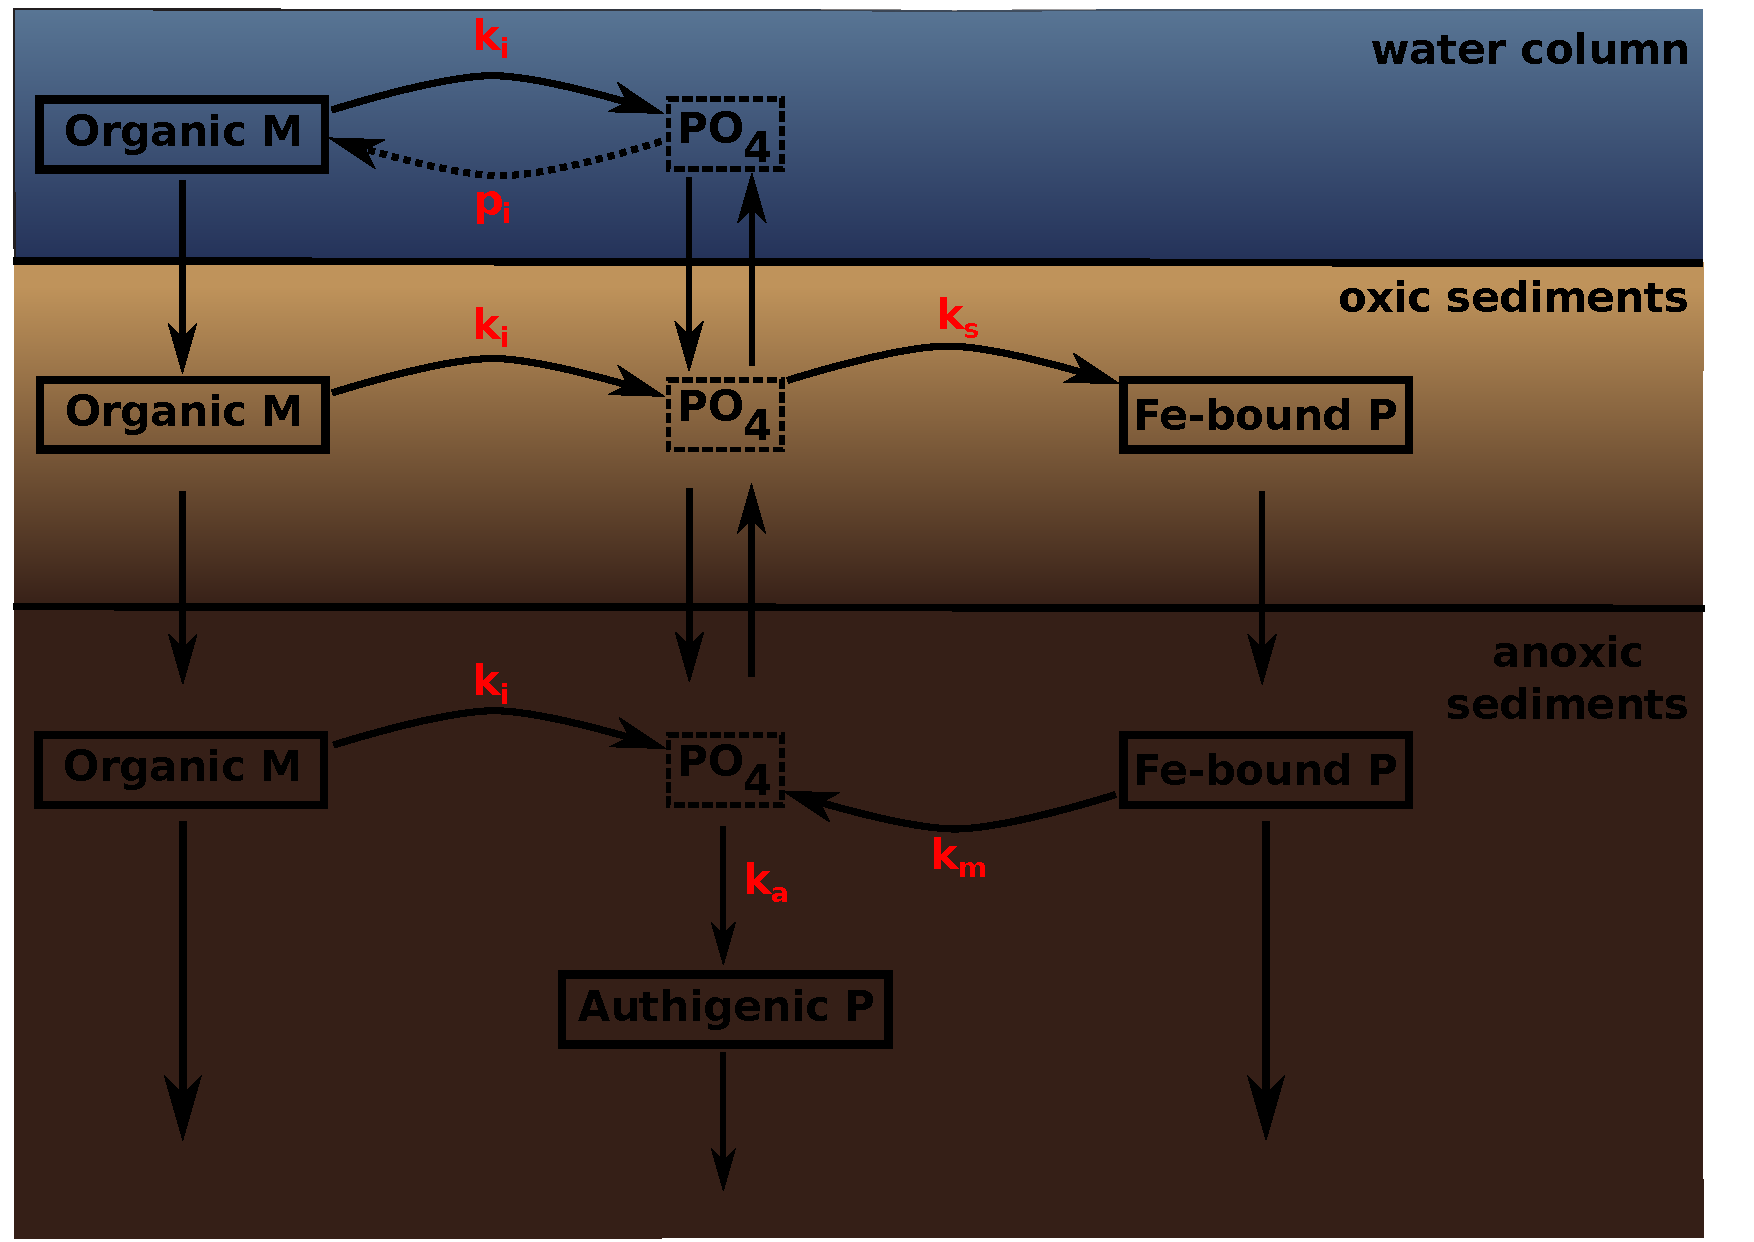
\includegraphics[width=0.8\textwidth]{figures/P-cycle.pdf}
	\caption{A schematic of the sedimentary P cycle in OMEN-SED (1.0). Red numbers represent kinetic rate constants for phosphorus dynamics (compare Table \ref{table:reaction_parameters}; p$_i$ represents uptake rate of PO$_4$ 
	via primary production in shallow environments). Adapted from \citet{caroline_p_slomp_key_1996}.}
	\label{fig:P-cycle}
	\end{center}
\end{figure}
To model phosphorus (P) in the sediments the model takes into account the change with depth of phosphate (PO$_4$) and iron-bound P, thereby mainly following the description of \citet{caroline_p_slomp_key_1996} 
and \citet{gypens_simple_2008}. Throughout the sediment column organic matter is mineralized resulting in a release of phosphate to the pore water. In the oxic part of the sediment, this PO$_4$ either 
diffuses upward to the water column or is adsorped to Fe oxides forming Fe-bound P (or M)\citep{slomp1998role}. In the suboxic/anoxic zone, PO$_4$ is not only produced through organic matter degradation but is 
also released from the Fe-bound P pool due to the reduction of Fe oxides. Furthermore, phosphate concentrations can become high enough in this layer for authigenic mineral formation to occur \citep{cappellen_mathematical_1988}. 
This phosphorus bound in authigenic minerals represents a permanent sink for reactive phosphorus \citep{caroline_p_slomp_key_1996}. See Figure \ref{fig:P-cycle} for a schematic overview of the sedimentary P cycle.
Therefore the diagenetic equations for phosphorus are written:
\begin{align}
\intertext{1. Layer ($z \leq z_{\mathrm{ox}}$)}
 \frac{\partial \chem{PO_4}^I}{\partial t} &= \frac{D_{\chem{PO_4}}}{1+K_{\chem{PO_4}}^I} \frac{\partial^2\chem{PO_4}^I }{\partial z^2} - w\frac{\partial \chem{PO_4}^I }{\partial z} + \frac{1-\phi}{\phi}\frac{1}{1+K_{\chem{PO_4}}^I}\sum_i 
					\left( \chem{PC}_i \cdot k_i \cdot C_{i}(z) \right) \notag\\
					& - \frac{k_{s}}{1+K_{\chem{PO_4}}^I}(\chem{PO_4}^I-\chem{PO_4}^s)\label{eq:PO4_ODE_L1}\\  %&\text{1. Layer ($z\leq z_{\mathrm{ox}} \leq zbio$)}\label{eq:SO4_ODE1_Case1_sub1}\\
 \frac{\partial M^I}{\partial t} &= D_{M}\frac{\partial^2M^I }{\partial z^2} - w\frac{\partial M^I }{\partial z} + \frac{\phi}{1-\phi}k_{s}(\chem{PO_4}^I-\chem{PO_4}^s)\label{eq:M_ODE_L1}\\  
 \intertext{2. Layer ($z_{\mathrm{ox}} < z$)} 
 \frac{\partial M^{II}}{\partial t} & = D_{M}\frac{\partial^2M^{II} }{\partial z^2} - w\frac{\partial M^{II} }{\partial z} - k_{m}(M^{II} - M^\infty)\label{eq:M_ODE_L2}\\  
 \frac{\partial \chem{PO_4}^{II}}{\partial t} &= \frac{D_{\chem{PO_4}}}{1+K_{\chem{PO_4}}^{II}} \frac{\partial^2\chem{PO_4}^{II} }{\partial z^2} - w\frac{\partial \chem{PO_4}^{II} }{\partial z} + \frac{1-\phi}{\phi} \frac{1}{1+K_{\chem{PO_4}}^{II}}\sum_i 
					\left( \chem{PC}_i \cdot k_i \cdot C_{i}(z) \right) \notag\\
					& - \frac{k_{a}}{1+K_{\chem{PO_4}}^{II}}(\chem{PO_4}^{II}-\chem{PO_4}^a) + \frac{(1-\phi)}{\phi}\frac{k_{m}}{1+K_{\chem{PO_4}}^{II}}(M^{II}-M^\infty)\label{eq:PO4_ODE_L2}\\
\end{align}
% where
% \begin{align}
%  D_{\chem{PO_4}}&=D_{\chem{PO_4}, 0}+D_{\mathrm{bio}} &\text{ and }\quad D_{M}&= D_{\mathrm{bio}} &\text{if ($z\leq z_{\mathrm{bio}}$)}\\
%  D_{\chem{PO_4}}&=D_{\chem{PO_4}, 0} &\text{ and }\quad D_{M}&= 0 &\text{if ($z > z_{\mathrm{bio}}$)} 
% \end{align}
The boundary conditions to solve Equations \ref{eq:PO4_ODE_L1} - \ref{eq:PO4_ODE_L2} are summarized in Table \ref{Tab:BC_PO4+M}. 
The model assumes known bottom water concentrations and equal concentrations and diffusive fluxes at $z_{\mathrm{bio}}$ and $z_{\mathrm{ox}}$ for both species. Additionally it considers no change in phosphate flux and an assymptotic Fe-bound P 
concentration at $z_\infty$. \\

\textcolor{red}{@ Sandra: SWI Flux for M does not exist, right???}

\begin{table}[tbp]
\caption{Boundary conditions for phosphate and Fe-bound P (M).}
% title of Table
\centering
% used for centering table
\begin{tabular}{ |l| l| l|}
\hline
\textbf{Boundary}& \textbf{Condition}&\\
\hline
$z=0$& known concentration& 1) \chem{PO_4}(0)=\chem{PO_{40}}  \\
$z=z_{\mathrm{bio}}$&continuity& 2) $\chem{PO_4}(z_{\mathrm{bio}}^-)$=$\chem{PO_4}(z_{\mathrm{bio}}^+)$\\
               & flux & 3) $\left(D_{\chem{PO_4},0}+D_{\mathrm{bio}}\right )\cdot \frac{\partial \chem{PO_4}}{\partial z}|_{z_{\mathrm{bio}}^-}=D_{\chem{PO_4},0} \cdot \frac{\partial \chem{PO_4}}{\partial z}|_{z_{\mathrm{bio}}^+}$\\
$z=z_{\mathrm{ox}}$& continuity& 4) $\chem{PO_4}(z_{\mathrm{ox}}^-)$=$\chem{PO_4}(z_{\mathrm{ox}}^+)$\\
               & flux & 5) $-\frac{D_{\chem{PO_4}}}{1+K_{\chem{PO_4}}^I} \cdot \frac{\partial \chem{PO_4}}{\partial z}|_{z_{\mathrm{ox}}^-} =-\frac{D_{\chem{PO_4}}}{1+K_{\chem{PO_4}}^{II}} \cdot \frac{\partial \chem{PO_4}}{\partial z}|_{z_{\mathrm{ox}}^+}$\\
%&where:\textcolor{red}{$\int_{z_{\chem{SO_4}}}^{\infty}$ here?} & $\quad F_{\chem{H_2S}}(z_{\mathrm{ox}})=\frac{1-\phi}{\phi} \cdot \textcolor{red}{\gamma_{\chem{H_2S}}\cdot} \left( \int_{z_{\chem{NO_3}}}^{SO_4}  \sum_i SO_4C \cdot k_i \cdot C_i\ dz + \gamma_{CH_4}\cdot \int_{z_{\chem{SO_4}}}^{\infty}  \sum_i SO_4C \cdot k_i \cdot C_i\ dz \right)$\\          
$z=z_{\infty}$& flux & 10) $\frac{\partial \chem{PO_4}}{\partial z}|_{z_\infty}=0$\\
\hline
$z=0$& known concentration& 1) $M(0)=M_0$  \\
$z=z_{\mathrm{bio}}$&continuity& 2) $M(z_{\mathrm{bio}}^-)$=$M(z_{\mathrm{bio}}^+)$\\
  & flux & 3) $\frac{\partial M}{\partial z}|_{z_{\mathrm{bio}}^-}=\frac{\partial M}{\partial z}|_{z_{\mathrm{bio}}^+}$\\
$z=z_{\mathrm{ox}}$& continuity& 4) $M(z_{\mathrm{ox}}^-)$=$M(z_{\mathrm{ox}}^+)$\\
  & flux & 5) $\frac{\partial M}{\partial z}|_{z_{\mathrm{ox}}^-} =\frac{\partial M}{\partial z}|_{z_{\mathrm{ox}}^+}$\\
%&where:\textcolor{red}{$\int_{z_{\chem{SO_4}}}^{\infty}$ here?} & $\quad F_{\chem{H_2S}}(z_{\mathrm{ox}})=\frac{1-\phi}{\phi} \cdot \textcolor{red}{\gamma_{\chem{H_2S}}\cdot} \left( \int_{z_{\chem{NO_3}}}^{SO_4}  \sum_i SO_4C \cdot k_i \cdot C_i\ dz + \gamma_{CH_4}\cdot \int_{z_{\chem{SO_4}}}^{\infty}  \sum_i SO_4C \cdot k_i \cdot C_i\ dz \right)$\\          
$z=z_{\infty}$& assymptotic concentration & 10) $M(z_\infty)=M_\infty$\\
\hline    
\end{tabular}
\label{Tab:BC_PO4+M}
% is used to refer this table in the text
\end{table}
% \subsubsection{Sulfide}
% Processes considered\\
% general equation\\
% solution\\

\subsubsection{Dissolved Inorganic Carbon (DIC)}
Dissolved inorganic carbon (DIC) is produced by when organic matter is degraded. Explain different ratios for the two layers.
\begin{align}
\intertext{1. Layer ($z \leq z_{\chem{SO_4}}$)}
  \frac{\partial DIC^I}{\partial t} &= 0 = D_{DIC} \frac{\partial^2DIC^I }{\partial z^2} - w\frac{\partial DIC^I }{\partial z} + \frac{1-\phi}{\phi} \cdot \sum_i \chem{DICC^I} \cdot k_i \cdot C_{i}(z)\label{eq:DIC_ODE1_L1}\\ %\qquad &\text{1. Layer ($z\leq z_{\mathrm{ox}}$)}\\
 \intertext{2. Layer ($z_{\chem{SO_4}} < z \leq z_\infty$)} 
  \frac{\partial DIC^{II}}{\partial t} &= 0 = D_{DIC} \frac{\partial^2DIC^{II} }{\partial z^2} - w\frac{\partial DIC^{II} }{\partial z} + \frac{1-\phi}{\phi} \cdot \sum_i \chem{DICC^{II}} \cdot k_i \cdot C_{i}(z)\label{eq:DIC_ODE1_L2} %\qquad &\text{1. Layer ($z\leq z_{\mathrm{ox}}$)}\\
\end{align}
To solve equations \ref{eq:DIC_ODE1_L1} and \ref{eq:DIC_ODE1_L2} the model assumes the boundary conditions summarised in Table \ref{Tab:BC_DIC+ALK}.

\begin{table}[tbp]
\caption{Boundary conditions for DIC and alkalinity.}
% title of Table
\centering
% used for centering table
\begin{tabular}{ |c| c| c l|}
\hline
\textbf{Boundary}& \textbf{Condition}&&\\
\hline
$z=0$& known concentration& 1)& $\chem{DIC}(0)=\chem{DIC}_{0}$  \\
$z=z_{\mathrm{bio}}$&continuity& 2)& $\chem{DIC}(z_{\mathrm{bio}}^-)$=$\chem{DIC}(z_{\mathrm{bio}}^+)$\\
               & flux & 3)& $-\left(D_{\chem{DIC},0}+D_{\mathrm{bio}}\right )\cdot \frac{\partial \chem{DIC}}{\partial z}|_{z_{\mathrm{bio}}^-}=-D_{\chem{DIC},0} \cdot \frac{\partial \chem{DIC}}{\partial z}|_{z_{\mathrm{bio}}^+}$\\
$z=z_{\chem{SO_4}}$& continuity & 8)& $\chem{DIC}(z_{\chem{SO_4}}^-)$=$\chem{DIC}(z_{\chem{SO_4}}^+)$\\ %$\frac{\partial \chem{DIC}}{\partial z}|_{z_{\chem{DIC}}}=0$\\
               & flux (with AOM) & 9)&  $-D_{\chem{DIC}}\cdot \frac{\partial \chem{DIC}}{\partial z}|_{z_{\chem{SO_4}}^-} + \gamma_\chem{CH_4}\cdot F_{\chem{CH_4}}(z_{\chem{SO_4}})=-D_{\chem{DIC}} \cdot \frac{\partial \chem{DIC}}{\partial z}|_{z_{\chem{SO_4}}^+}$\\
&where: & &$\quad F_{\chem{CH_4}}(z_{\chem{SO_4}})=\frac{1-\phi}{\phi} \cdot \int_{z_{\chem{SO_4}}}^{\infty}  \sum_i \chem{MC} \cdot k_i \cdot C_i\ dz$ \\          
$z=z_{\infty}$& zero \chem{DIC} flux & 10)& $\frac{\partial \chem{DIC}}{\partial z}|_{z_\infty}=0$\\
\hline
$z=0$& known concentration& 1)& $\chem{ALK}(0)=\chem{ALK}_{0}$  \\
$z=z_{\mathrm{bio}}$&continuity& 2)& $\chem{ALK}(z_{\mathrm{bio}}^-)$=$\chem{ALK}(z_{\mathrm{bio}}^+)$\\
               & flux & 3)& $-\left(D_{\chem{ALK},0}+D_{\mathrm{bio}}\right )\cdot \frac{\partial \chem{ALK}}{\partial z}|_{z_{\mathrm{bio}}^-}=-D_{\chem{ALK},0} \cdot \frac{\partial \chem{ALK}}{\partial z}|_{z_{\mathrm{bio}}^+}$\\
$z=z_{\mathrm{ox}}$& continuity& 4)& $\chem{ALK}(z_{\mathrm{ox}}^-)$=$\chem{ALK}(z_{\mathrm{ox}}^+)$\\
               & flux & 5)& $-D_{\chem{ALK}} \cdot \frac{\partial \chem{ALK}}{\partial z}|_{z_{\mathrm{ox}}^-} +  F_{\chem{ALK}}(z_{\mathrm{ox}})=-D_{\chem{ALK}} \cdot \frac{\partial \chem{ALK}}{\partial z}|_{z_{\mathrm{ox}}^+}$\\
&where: & &$\quad F_{\chem{ALK}}(z_{\mathrm{ox}})=\frac{1-\phi}{\phi} \cdot \left( \chem{ALK}^\chem{H_2S}\gamma_\chem{H_2S} \int_{z_{\chem{NO_3}}}^{\chem{SO_4}} \sum_i \chem{SO_4C} \cdot k_i \cdot C_i\ dz \right)+ $\\
& & &$\qquad \qquad \qquad \quad \frac{1-\phi}{\phi} \cdot \left(\chem{ALK}^\chem{NIT} \frac{\gamma_\chem{NH_4}}{1+k_\chem{NH_4}}\int_{z_{\chem{NO_3}}}^{\infty}  \sum_i \chem{NC_i} \cdot k_i \cdot C_i\ dz \right)$\\            
$z=z_{\chem{NO_3}}$&continuity& 6)& $\chem{ALK}(z_{\chem{NO_3}}^-)$=$\chem{ALK}(z_{\chem{NO_3}}^+)$\\
               & flux & 7)& $-D_{\chem{ALK}}\cdot \frac{\partial \chem{ALK}}{\partial z}|_{z_{\chem{NO_3}}^-}=-D_{\chem{ALK}} \cdot \frac{\partial \chem{ALK}}{\partial z}|_{z_{\chem{NO_3}}^+}$\\
$z=z_{\chem{SO_4}}$& continuity & 8)& $\chem{ALK}(z_{\chem{SO_4}}^-)$=$\chem{ALK}(z_{\chem{SO_4}}^+)$\\ %$\frac{\partial \chem{ALK}}{\partial z}|_{z_{\chem{ALK}}}=0$\\
               & flux (with AOM) & 9)&  $-D_{\chem{ALK}}\cdot \frac{\partial \chem{ALK}}{\partial z}|_{z_{\chem{SO_4}}^-} + F_{\chem{ALK}}(z_{\chem{SO_4}})=-D_{\chem{ALK}} \cdot \frac{\partial \chem{ALK}}{\partial z}|_{z_{\chem{SO_4}}^+}$\\
&where: & &$\quad F_{\chem{ALK}}(z_{\chem{SO_4}})=\frac{1-\phi}{\phi} \cdot \left( \chem{ALK}^\chem{AOM}\gamma_\chem{CH_4}\cdot \int_{z_{\chem{SO_4}}}^{\infty}  \sum_i \chem{MC} \cdot k_i \cdot C_i\ dz \right)$ \\          
$z=z_{\infty}$& zero \chem{ALK} flux & 10)& $\frac{\partial \chem{ALK}}{\partial z}|_{z_\infty}=0$\\
\hline    
\end{tabular}
\label{Tab:BC_DIC+ALK}
\end{table}

\subsubsection{Alkalinity}
Alkalinity is produced and consumed by when organic matter is degraded. Explain why it is produced/consumed, where and how in the different layers $j \in \{I,\ II,\ III,\ IV\}$ and talk earlier on in the model description why it matters.
% \begin{equation}
%   \frac{\partial \chem{ALK}^{}}{\partial t} = 0 = D_{\chem{ALK}} \frac{\partial^2\chem{ALK}^{I} }{\partial z^2} - w\frac{\partial \chem{ALK}^{I} }{\partial z} + \frac{1-\phi}{\phi} \cdot \sum_i \mathrm{REAC_{ALK}} \cdot k_i \cdot C_{i}(z) \label{eq:ALK_ODE}
% \end{equation}
\begin{align}
 \intertext{1. Layer ($z \leq z_{\chem{ox}}$)} 
\frac{\partial \chem{ALK}^{I}}{\partial t} &= 0 = D_{\chem{ALK}} \frac{\partial^2\chem{ALK}^{I} }{\partial z^2} - w\frac{\partial \chem{ALK}^{I} }{\partial z} + \frac{1-\phi}{\phi} \cdot \sum_i (\gamma_{\chem{NH_4}} \chem{NC_i} \chem{ALK}^\mathrm{NIT} + \chem{ALK}^\mathrm{OX})\cdot k_i \cdot C_{i}(z) \label{eq:ALK_ODE1_L1}\\
 \intertext{2. Layer ($z_{\chem{ox}} < z \leq z_{\chem{NO_3}} $)} 
\frac{\partial \chem{ALK}^{II}}{\partial t} &= 0 = D_{\chem{ALK}} \frac{\partial^2\chem{ALK}^{II} }{\partial z^2} - w\frac{\partial \chem{ALK}^{II} }{\partial z} + \frac{1-\phi}{\phi} \cdot \sum_i \chem{ALK}^\mathrm{DEN}\cdot k_i \cdot C_{i}(z)\label{eq:ALK_ODE1_L2}
 \intertext{3. Layer ($z_{\chem{NO_3}} < z \leq z_{\chem{SO_4}} $)} 
\frac{\partial \chem{ALK}^{III}}{\partial t} &= 0 = D_{\chem{ALK}} \frac{\partial^2\chem{ALK}^{III} }{\partial z^2} - w\frac{\partial \chem{ALK}^{III} }{\partial z} + \frac{1-\phi}{\phi} \cdot \sum_i \chem{ALK}^\mathrm{SUL}\cdot k_i \cdot C_{i}(z)\label{eq:ALK_ODE1_L2}
 \intertext{4. Layer ($z_{\chem{SO_4}} < z \leq z_{\infty} $)} 
\frac{\partial \chem{ALK}^{IV}}{\partial t} &= 0 = D_{\chem{ALK}} \frac{\partial^2\chem{ALK}^{IV} }{\partial z^2} - w\frac{\partial \chem{ALK}^{IV} }{\partial z} + \frac{1-\phi}{\phi} \cdot \sum_i \chem{ALK}^\mathrm{MET}\cdot k_i \cdot C_{i}(z)\label{eq:ALK_ODE1_L2}
\end{align}
To solve equations \ref{eq:ALK_ODE1_L1} and \ref{eq:ALK_ODE1_L2} the model assumes the boundary conditions summarised in Table \ref{Tab:BC_DIC+ALK}.


\subsection{Model Parameters}
This section describes the parameters used in OMEN-SED (1.0) to describe sediment transport and biogeochemical reactions related to the burial and mineralization of organic matter under a wide range of environmental conditions. 
Table \ref{table:sed-charac_transport-parameters} states the parameters for sediment characteristics and Table \ref{table:reaction_parameters} summarizes the stoichiometric factors and 
secondary reaction parameters used in the model.

\subsubsection{Transport Parameters}
Advection is the bulk flow of sediments and can be directly related to the accumulation of new material on the seafloor \citep[i.e. sedimentation,][]{burdige2006geochemistry}. 
This results in a downward flux of older sediment material and porewater in relation to the sediment-water interface. OMEN-SED (1.0) uses the empirical global relationship between 
sediment accumulation rate (cm yr$^{-1}$) and seafloor depth (m) of \citet{middelburg_empirical_1997}: 
\begin{equation}
 w = 3.3\cdot 10^{-0.87478367-0.00043512\cdot \text{depth}}\label{eq:sedimentation_rate}
\end{equation}
As discussed before (Sec. \ref{subsec:Transport}), the diffusion coefficient of species $i$ is calculated as $D_i=D_{i,0}+D_{\mathrm{bio}}=D_{\mathrm{mol},i}\cdot f_{ir}+D_{\mathrm{bio}}$ for dissolved species and $D_i=D_{\mathrm{bio}}$ for solid species. 
The bioturbation coefficient $D_{\mathrm{bio}}$ (cm$^2$ yr$^-1$) is constant in the bioturbated zone and also follows the empirical relationship by \citet{middelburg_empirical_1997}:
\begin{equation}
 D_{\mathrm{bio}} = 5.2\cdot 10^{0.76241122-0.00039724\cdot \text{depth}}\label{eq:bioturbation_coeff}
\end{equation}
Studies showed that bioturbational effects on a global scale are largely restricted to the upper 10 cm of the sediments and are only marginally related to seafloor depth \citep[e.g.][]{boudreau_mean_1998, teal_global_2010}. 
Therefore, OMEN-SED (1.0) imposes a globally invariant bioturbation depth of 10 cm. 
Bioirrigation can enhance the molecular diffusion coefficient $D_{i,0}=D_{\mathrm{mol},i}\cdot f_{ir}$ \citep{soetaert1996dynamic}. However, here we do not consider this effect 
and set $f_{ir}$ to a constant value of 1. The specific molecular diffusion coefficients $D_{\mathrm{mol},i}$ are corrected for sediment porosity $\phi$, tortuosity F and are linearly interpolated for an ambient temperature $T$ using zero-degree 
coefficients $D^0_i$ and temperature dependent diffusion coefficients $D^T_i$ \citep[compare ][]{gypens_simple_2008}:
\begin{equation*}
 D_{\mathrm{mol},i} = (D^0_i + D^T_i \cdot T )\cdot \frac{1}{\phi\cdot F}
\end{equation*}
Tortuosity can be expresssed in terms of porosity as $F = \frac{1}{\phi^m}$ \citep{ullman_diffusion_1982} with the exponent $m$ varying according to the type of sediment (here we use m=3). 
%\textcolor{red}{in matlab: $\phi^{tort-1}$; but see Gypens et al. (2008) the exponent is a parameter m not tortuosity...??}
Values for $D^T_i$ and $D^0_i$ are summarized in Table \ref{table:sed-charac_transport-parameters} and are adapted from \citet{Li_diffusion_1974} and \citet{gypens_simple_2008}.

\begin{table}[hbtp]
\caption{Fixed sediment characteristics and transport parameters. \textcolor{red}{TODO: Update table!}}
% title of Table
\centering
% used for centering table
\begin{tabular}{l c c l}
% centered columns (6 columns)
\hline\hline
%inserts double horizontal lines
Parameter & Unit  & Value & Description/Source\\
\hline
$\rho_{\mathrm{sed}}$ & g\,cm$^{-3}$ & 2.5 & Sediment density \\
$w$ & cm\,yr$^{-1}$ &  Fct. of seafloor  & Advection/Sediment accumulation rate \\
&& depth & \citet{middelburg_empirical_1997}\\
$z_{\mathrm{bio}}$& cm & 10 & Bioturbation depth\\
&&&\citet{boudreau_mean_1998, teal_global_2010}\\
$D_{\mathrm{bio}}$& cm$^2$\,yr$^{-1}$ & Fct. of seafloor & Bioturbation coefficient\\
&& depth &\citet{middelburg_empirical_1997}\\
$\phi$ & - & 0.8 & Porosity\\
F & - &  $\frac{1}{\phi^m}$ & Tortuosity, here m=3\\
f$_{ir}$ & - & 1 & Irrigation factor\\
%dispF & - & $irrF \cdot \phi^{F-1.0}$ & Dispersion factor\\
$\chem{PO_4}^s$ & mol\,cm$^{-3}$ & $1\cdot 10^{-9}$ & equilibrium conc. for P sorption\\
&&&\citet{caroline_p_slomp_key_1996}\\
$\chem{PO_4}^a$ & mol\,cm$^{-3}$ & $3.7\cdot 10^{-9}$ & equilibrium conc. for authigenic P precipitation\\
&&&\citet{caroline_p_slomp_key_1996}\\
$\chem{M}^\infty$ & mol\,cm$^{-3}$ & \textcolor{red}{$1.99\cdot 10^{-9}$} & asymptotic concentration for Fe-bound P\\
&&&\citet{caroline_p_slomp_key_1996}\\
\multicolumn{4}{l}{\textbf{Diffusion coefficients} \citep{Li_diffusion_1974, gypens_simple_2008}}\\
$D_{\chem{O_2}}^0$ & cm$^2$\,yr$^{-1}$ & 348.62172 &Molecular diffusion coefficient of oxygen at 0$^\circ$C\\
$D_{\chem{O_2}}^T$ & cm$^2$\,yr$^{-1}$\,${}^{\circ}$C$^{-1}$ & 14.08608 &Diffusion coefficient for linear temp. dependence of oxygen\\ % value was 0.0386 (changed by Nicolas 2207)
$D_{\chem{NO_3}}^0$ & cm$^2$\,yr$^{-1}$ & 308.42208 &Molecular diffusion coefficient of nitrate at 0$^\circ$C\\
$D_{\chem{NO_3}}^T$ & cm$^2$\,yr$^{-1}$\,${}^{\circ}$C$^{-1}$ & 12.2640 &Diffusion coefficient for linear temp. dependence of nitrate\\ % value was 0.0386 (changed by Nicolas 2207)
$D_{\chem{NH_4}}^0$ & cm$^2$\,yr$^{-1}$ & 308.42208 &Molecular diffusion coefficient of ammonium at 0$^\circ$C\\
$D_{\chem{NH_4}}^T$ & cm$^2$\,yr$^{-1}$\,${}^{\circ}$C$^{-1}$ & 12.2640 &Diffusion coefficient for linear temp. dependence of ammonium\\ % value was 0.0386 (changed by Nicolas 2207)
$D_{\chem{SO_4}}^0$ & cm$^2$\,yr$^{-1}$ & 157.68 &Molecular diffusion coefficient of sulfate at 0$^\circ$C\\
$D_{\chem{SO_4}}^T$ & cm$^2$\,yr$^{-1}$\,${}^{\circ}$C$^{-1}$ & 7.884 &Diffusion coefficient for linear temp. dependence of sulfate\\ % value was 0.0386 (changed by Nicolas 2207)
$D_{\chem{H_2S}}^0$ & cm$^2$\,yr$^{-1}$ & 307.476 & Molecular diffusion coefficient of sulfide at 0$^\circ$C\\
$D_{\chem{H_2S}}^T$ & cm$^2$\,yr$^{-1}$\,${}^{\circ}$C$^{-1}$ & 9.636 & Diffusion coefficient for linear temp. dependence of sulfide\\ % value was 0.0386 (changed by Nicolas 2207)
$D_{\chem{PO_4}}^0$ & cm$^2$\,yr$^{-1}$ & 112.90764 &Molecular diffusion coefficient of phosphate at 0$^\circ$C\\
$D_{\chem{PO_4}}^T$ & cm$^2$\,yr$^{-1}$\,${}^{\circ}$C$^{-1}$ & 5.586252 &Diffusion coefficient for linear temp. dependence of phosphate\\ % value was 0.0386 (changed by Nicolas 2207)
\hline\hline
% inserts double horizontal lines
\end{tabular}
\label{table:sed-charac_transport-parameters}
% is used to refer this table in the text
\end{table}


\subsubsection {Reaction Parameters}
%The parameters relating to organic matter 
%The overall reactions implemented in OMEN-SED (1.0) are listed in Table \ref{table:reactions_processes}. 
The applied multi-G approach for organic matter degradation considers specific degradation rate constants $k_i$ (yr$^{-1}$) for each compound class. The degradation constants are generally taken from the coupled Earth System model 
and are assumed invariant along the sediment column, therefore independent of the nature of the terminal electron acceptor. 
The stoichiometry of organic matter is represented by the factors \chem{NC_i} and \chem{PC_i} denoting the molecular nitrogen to carbon and phosphorus to carbon ratio. 
In the sulfidic and methanic zone the 
reduction of 1 mol organic matter additionally produces 0.5 mol of hydrogen sulfide (\chem{SO_4C}) and 0.5 mol of methane (\chem{MC}). 
In the total sediment column organic matter mineralization consumes the specific terminal electron acceptor with a fixed ratio (\chem{OC}, \chem{NO_3C} and \chem{SO_4C} respectively). 
See Table \ref{table:reaction_parameters} for a complete summary of the parameters and their values.
% \textcolor{red}{Or bit longer:}\\
% In the sulfidic and methanic zone the 
% reduction of 1 mol organic matter additionally produces 0.5 mol of hydrogen sulfide (\chem{SO_4C}) and 0.5 mol of methane (\chem{MC}) respectively. 
% In the oxic part of the sediments 1 mol of oxygen is needed to mineralize 1 mol of organic matter (\chem{OC}). In the nitrate and sulfate reduction zone 1 mol of organic matter is reduced by 
% 0.8906 mol of nitrate (\chem{NO_3C}) and 0.5 mol of sulfate (\chem{SO_4C}) respectively. \\
%\textcolor{red}{Next bit from Gypens:} Re-oxidation occurs in a ratio of 1 mol of oxygen per mol of carbon anoxically mineralized. Similarly, 2 mol of oxygen
%are consumed during nitrification of \chem{NH_4} produced in the anoxic zone. As nitrification may be incomplete in the oxic layer, we similarly allow for part of the ammonium flux to escape re-oxidation. 
\begin{table}[btp]
\caption{Values for biogeochemical parameters used in OMEN-SED (1.0). 
%\textcolor{red}{Stoichiometric factor for oxygen and sulfate relates to mol of terminal electron acceptor consumed for 1 mol of organic matter mineralized. 
%NC and MC related to mol of reduced species produces per mol organic matter mineralized. correct???}
}
% title of Table
\centering
% used for centering table
\begin{tabular}{l c c l}
% centered columns (6 columns)
\hline\hline
%inserts double horizontal lines
Parameter/Variable & Unit  & Value & Description\\
\hline
\multicolumn{4}{l}{\textbf{Stoichiometric factors and molecular ratios}}\\
\chem{NC_1} & mol/mol & 0.1509 & nitrogen to carbon ratio\\
& & & \textcolor{red}{refractory fraction, two different ones? why these values?}\\
\chem{NC_2} & mol/mol & 0.13333 & nitrogen to carbon ratio\\
& & & labile fraction\\
\chem{PC_i} & mol/mol & 0.0094 & phosphorus to carbon ratio\\
\chem{MC}& mol/mol & 0.5 & methane to carbon ratio\\
&&&produced during methanogenesis\\
\chem{OC} & mol/mol & 1.0 & oxygen to carbon ratio\\
\chem{NO_3C} & mol/mol & 94.4/106 & nitrate to carbon ratio\\
\chem{SO_4C} & mol/mol & 0.5 & sulfate to carbon ratio\\
$\chem{ALK}^\mathrm{OX}$ & mol/mol & 15/106 & ALK from aerobic degradation\\
$\chem{ALK}^\mathrm{NIT}$ & mol/mol & -2 & ALK from nitrification\\
$\chem{ALK}^\mathrm{DEN}$ & mol/mol & 93.4/106 & ALK from denitrification\\
$\chem{ALK}^\mathrm{SUL}$ & mol/mol & 15/106 & ALK from sulfate reduction\\
$\chem{ALK}^\mathrm{MET}$ & mol/mol & 14/106 & ALK from methanogenesis\\
$\chem{ALK}^\mathrm{H2S}$ & mol/mol & -1 & ALK from \chem{H_2S} oxidation \textcolor{red}{CORRECT???}\\
$\chem{ALK}^\mathrm{AOM}$ & mol/mol & 2 & ALK from methanogenesis\\
%$DICC^I$ & $mol/mol$ & 1 & DIC to carbon ratio\\
%& & & until $z_{\chem{SO_4}}$\\
%$DICC^{II}$ & $mol/mol$ & 0.5 & DIC to carbon ratio\\
%& & & for methanogenesis\\[0.5ex]
\multicolumn{4}{l}{\textbf{Secondary reaction parameters}}\\
$\gamma_{\chem{NH_4}}$ & - & 0.8 & fraction of \chem{NH_4} that is oxidised\\
& & & in oxic layer\\
$\gamma_{\chem{H_2S}}$ & - & 0.95 & fraction of \chem{H_2S} that is oxidised\\
& & & in oxic layer\\
$\gamma_{\chem{CH_4}}$ & - & 1.0 & fraction of \chem{CH_4} that is oxidised\\
& & & at $z_{\chem{SO_4}}$\\
\multicolumn{4}{l}{\textbf{Rate constants}}\\
$k_i$ & yr$^{-1}$ & from Earth System Model & OM degradation rate constants\\
$k_s$ & yr$^{-1}$ & \textcolor{red}{???} & rate constant for P sorption\\
$k_m$ & yr$^{-1}$ & \textcolor{red}{???} & rate constant for Fe-bound P release\\
$k_a$ & yr$^{-1}$ & \textcolor{red}{???} & rate constant for authigenic P formation\\
\hline\hline
% inserts double horizontal lines
\end{tabular}
\label{table:reaction_parameters}
\end{table}

\subsection{Module Structure}
%Sandra: Technical description, e.g. how is it implemented and how can it be coupled to model\\
\textcolor{red}{TODO: }
%Describe in which order we calculate the different profiles/exchange fluxes (first calculating OM profile, then different TEA profiles).\\ 
An analytical steady-state solution is found for the reaction-transport equation of each chemical species in each layer. 
At each boundary (i.e. $z_{\mathrm{ox}}, z_{\mathrm{bio}}, z_{\chem{NO_3}}$ and $z_{\chem{SO_4}}$) the model has to match continuity and flux for different ODE solutions of the layer above and below the specific boundary. 
In particular the bioturbation boundary is problematic as it can theoretically occur in any geochemical layer. In order to simplify this recurring boundary matching problem it is implemented in an independent algorithm 
which is described in Section \ref{subsec:GBCM}. Instructions and requirements for coupling OMEN-SED (1.0) to a global Earth Sytem Model are given in Section \ref{subsubsec:ESM_coupling}.

\subsubsection{Generic boundary condition matching (GBCM)}\label{subsec:GBCM}
A general steady-state advection-diffusion-reaction (ADR) diagenetic equation looks like:
\begin{align} 
 \frac{\partial C}{\partial t} &= 0 = D\frac{\partial^2C }{\partial z^2} - w\frac{\partial C }{\partial z} - \sum_i \alpha_i \exp(-\beta_i z) - k\cdot C + Q.
\end{align}
where $z$ is the sediment depth, $t$ the time, $D$ is the diffusion coefficient and $w$ is the advection rate.\\
The ODE solution is of the general form:
\begin{align}
 C(z) &= A \exp(az) + B  \exp(bz) + \sum_i \frac{\alpha_i}{D \beta_i^2-w\beta_i-k}\cdot \exp(-\beta_i z) + \frac{Q}{k}
\end{align}
and can therefore be expressed as:
\begin{align}
C(z) = A \cdot E(z) + B \cdot F(z) + G(z) 
\end{align}
where $E(z)$, $F (z)$ are the homogeneous solutions of the ODE, G(z) the particular integral, and A, B are the integration constants.\\[1em]
Each boundary matching problem involves matching continuity and flux for the two solutions $C_U(z)$ (= 'upper') and $C_L(z)$ (= 'lower') across a boundary at $z = z_b$. Therefore, we get two ODE solutions of the genral form:
\begin{align}
C_U(z) &= A_U \cdot E_U(z) + B_U \cdot F_U(z) + G_U(z) \label{ODE_solution_U}\\
C_L(z) &= A_L \cdot E_L(z) + B_L \cdot F_L(z) + G_L(z) .\label{ODE_solution_L}
\end{align}
The two boundary conditions are: for continuity (where for generality we allow a discontinuity $V_b$) 
\begin{align}
  C_U(z_b) &= C_L(z_b) + V_b	\\
\intertext{and for flux}
 D_U C_U'(z_b) + wC_U(z_b) &=  D_LC_L'(z_b) + wC_L(z_b) + F_b
\end{align}
where $w$ is advection, $D$ are the diffusion coefficients and $F_b$ is any flux discontinuity.\\[1em]
In terms of the ODE solutions (\ref{ODE_solution_U}), (\ref{ODE_solution_L}), the boundary conditions represent two equations connecting the four integration constants:\\
\begin{equation}
 \begin{pmatrix} E_U & F_U \\ D_UE_U' & D_UF_U' \end{pmatrix} \begin{pmatrix} A_U \\ B_U \end{pmatrix} = \begin{pmatrix} E_L & F_L \\ D_LE_L' & D_LF_L' \end{pmatrix} \begin{pmatrix} A_L \\ B_L \end{pmatrix} 
 + \begin{pmatrix} G_L - G_U + V_b \\ D_LG_L' - D_UG_U' + F_b - wV_b\end{pmatrix} \label{Solution_BC}
\end{equation}
where the ODE solutions $E,\ F,\ G$ are all evaluated at $z_b$.\\[1em]
Equation (\ref{Solution_BC}) can be solved to give $A_U$ and $B_U$ as a function of the integration constants from the layer below ($A_L$ and $B_L$), thereby constructing a piecewise solution for the whole region, 
with now just two integration constants $A_L$ and $B_L$. \\[1em]
In the code the function \textsf{\textbf{benthic\_utils.matchsoln}} provides this solution in the form:
\begin{equation}
\begin{pmatrix} A_U \\ B_U \end{pmatrix} = \begin{pmatrix} c_1 & c_2 \\ c_3 & c_4 \end{pmatrix} \begin{pmatrix} A_L \\ B_L \end{pmatrix} + \begin{pmatrix} d_1 \\ d_2 \end{pmatrix} . \label{Solution_matchsoln} 
\end{equation}
Using (\ref{Solution_matchsoln}) we can now rewrite $C_U(z)$ in (\ref{ODE_solution_U}) as a function of $A_L$ and $B_L$:
\begin{equation*}
 C_U(z) = (c_1 A_L + c_2 B_L + d_1) \cdot E_U(z) + (c_3 A_L + c_4 B_L + d_2) \cdot F_U(z) + G_U(z) 
\end{equation*}
and hence define the ``transformed'' basis functions $E_U^*(z),\ F_U^*(z),\ G_U^*(z)$ such that:
\begin{equation}
 C_U(z) = A_L \cdot E_U^*(z) + B_L \cdot F_U^*(z) + G_U^*(z) \label{Solution_Upper_transformed_basis_fct}
\end{equation}
where
\begin{align}
 E_U^*(z) &= c_1 E_U(z) + c_3 F_U(z) \notag\\
 F_U^*(z) &= c_2 E_U(z) + c_4 F_U(z) \label{Solution_NEW_EFG}\\
 G_U^*(z) &= G_U(z) + d_1 E_U(z) + d_2 F_U(z) \notag
\end{align}
(in the code this is done by \textsf{\textbf{benthic\_utils.xformsoln}}).

%\subsubsection*{Application in the model}\label{subsubsec:GBCM-Appl}

\subsubsection*{Solving the sediment layer stack}
Equations (\ref{Solution_matchsoln}), (\ref{Solution_Upper_transformed_basis_fct}) and (\ref{Solution_NEW_EFG}) can now be applied for each layer boundary, working up from the bottom of the sediments. 
The net result is to construct a piecewise solution with just two integration constants (coming from the lowest layer), which can then be solved for by applying one boundary condition for the sediment-water interface 
and one for the bottom of the sediments (e.g. a concentration condition at the bottom of the sediments, and a flux condition at the SWI).

\textbf{\textcolor{red}{TODO: Add figure, illustrating this e.g. for nitrate...}}% The key point here is that this is now an algorithm (rather than a fully-worked-out algebraic solution),
% which only ever has to solve a two-simultaneous-equation problem as above.

\subsubsection*{Abstracting out the bioturbation boundary}
The bioturbation boundary affects the diffusion coefficient of the modelled solutes and the conservation equation of organic matter which is available for mineralization. 
The boundary is particularly inconvenient as it can in principle occur in the middle of any ``geochemical'' layer and therefore generates multiple cases. 
To simplify this for solutes, the ``piecewise solution construction'' above is used to abstract out the bioturbation boundary. 
An initial test for each layer is made to identify its ``bioturbation-status'' (fully bioturbated, fully non-bioturbated or crossing the bioturbation boundary) and (if needed) a piecewise solution is 
constructed by matching boundary conditions across the bioturbation boundary. 
The ``outside'' code therefore never needs to know whether it is dealing with a piecewise solution (i.e. matched across a bioturbation boundary) or a ``simple'' solution (i.e. the layer is fully bioturbated
or fully non-bioturbated).\\[1em]
In the code, this is performed by \textsf{\textbf{zTOC.prepfg\_l12}} which hands back a structure \textsf{ls} containing the ``bioturbation-status'' for each layer and (if needed) 
the description of the piecewise solution (coeffcients $c_1, c_2, c_3, c_4, d_1, d_2$ as above). So e.g. for sulfate, \textsf{\textbf{zTOC.prepfg\_l12}} is called three times at the beginning of \textsf{\textbf{zSO4.calcbc}} 
(one for each ``geochemical'' layer: oxic, suboxic, sulfidic) handing back three structures \textsf{ls} describing the layer's ``bioturbation-status'', abstracting away the bioturbation boundary and all associated conditional logic. 
When calculating the solutions for the different layers, the pre-calculated structure \textsf{ls} is passed to the function \textsf{\textbf{zTOC.calcfg\_l12}} which sorts out the correct
solution type to use.

\subsubsection{Coupling to an Earth System Model}\label{subsubsec:ESM_coupling}


\section {Test Cases}
\subsection{Benthic fluxes on a global scale}
Application to Seitert, 2004 OM, burwiczk see rate data and evaluation based on global data (Archer)

\subsection{HILDA-like test}

\subsection{GENIE-Cretaceous test?}

\section{Scope of applicability and model limitations}



\conclusions  %% \conclusions[modified heading if necessary]
TEXT

\section {Code Availability}


\appendix
\section{Reaction Network}    %% Appendix A
\begin{sidewaystable}[tbp]
\caption{Primary pathways of organic matter degradation, secondary redox reactions and stoichiometries implemented in the reaction network.}
% title of Table
\centering
% used for centering table
\begin{tabular}{l l}
% centered columns (6 columns)
\hline\hline
%inserts double horizontal lines
 Pathway & Stoichiometry \\
\hline
& Primary Redox Reactions\\
\hline
Aerobic degradation &  $ \chem{(CH_2O)_x(NH_3)_y(H_3PO_4)_z} + \mathrm{(x+2y)}\chem{O_2} + \mathrm{(y+2z)}\chem{HCO_3^-} \rightarrow \mathrm{(x+y+2z)}\chem{CO_2} + \chem{yNO_3^-} + \chem{zHPO_4^{2-}} + \mathrm{(x+2y+2z)}\chem{H_2O}$\\
Denitrification & $ 5\chem{(CH_2O)_x(NH_3)_y(H_3PO_4)_z} + \mathrm{(4x+3y)}\chem{NO_3^-} \rightarrow \mathrm{(2x+4y)}\chem{N_2} +  \mathrm{(x-3y+10z)}\chem{CO_2} + \mathrm{(4x+3y-10z)}\chem{HCO_3^-} + 5\chem{zHPO_4^{2-}} + \mathrm{(3x+6y+10z)}\chem{H_2O}$\\
Sulfate reduction &  $ 2\chem{(CH_2O)_x(NH_3)_y(H_3PO_4)_z} + \chem{xSO_4^{2-}} +  \mathrm{2(y-2z)}\chem{CO_2} + \mathrm{2(y-2z)}\chem{H_2O}\rightarrow \chem{xH_2S} +  \mathrm{2(x+y-2z)}\chem{HCO_3^-}  + \mathrm{2y}\chem{NH_4^+} + 2\chem{zHPO_4^{2-}}$\\
Methanogenesis & -----\\
\hline
& Secondary Redox Reactions\\
\hline
Nitrification & $\chem{NH_4^++2O_2+2HCO_3^-}\rightarrow \chem{NO_3^-+2CO_2+3H_2O}$\\
Sulfide oxidation & $\chem{H_2S + 2O_2 + 2HCO_3^-} \rightarrow \chem{SO_4^{2-} + 2CO_2 + 2H_2O}$\\
AOM & $\chem{CH_4 + SO_4^{2-}} \rightarrow \chem{HCO_3^- + HS^- + H_2O}$ \textcolor{red}{how get $H_2S$?} $\rightarrow \chem{CO_3^{2-}+H_2S+H_2O}$\\
\hline\hline
% inserts double horizontal lines
\end{tabular}
\label{table:Reaction_Network}
% is used to refer this table in the text
\end{sidewaystable}


\subsection{}                               %% Appendix A1, A2, etc.




\begin{acknowledgements}
TEXT
\end{acknowledgements}


%% REFERENCES

%% The reference list is compiled as follows:

\newpage
\bibliographystyle{apalike} %Style of Bibliography: plain / apalike / amsalpha / ...
%\bibliography{/home/alex/BRL/bib/literature/VORbib.bib} %You need a file 'literature.bib' for this.
\bibliography{Sediment_model}


%% Since the Copernicus LaTeX package includes the BibTeX style file copernicus.bst,
%% authors experienced with BibTeX only have to include the following two lines:
%%
%% \bibliographystyle{copernicus}
%% \bibliography{example.bib}
%%
%% URLs and DOIs can be entered in your BibTeX file as:
%%
%% URL = {http://www.xyz.org/~jones/idx_g.htm}
%% DOI = {10.5194/xyz}


%% LITERATURE CITATIONS
%%
%% command                        & example result
%% \citet{jones90}|               & Jones et al. (1990)
%% \citep{jones90}|               & (Jones et al., 1990)
%% \citep{jones90,jones93}|       & (Jones et al., 1990, 1993)
%% \citep[p.~32]{jones90}|        & (Jones et al., 1990, p.~32)
%% \citep[e.g.,][]{jones90}|      & (e.g., Jones et al., 1990)
%% \citep[e.g.,][p.~32]{jones90}| & (e.g., Jones et al., 1990, p.~32)
%% \citeauthor{jones90}|          & Jones et al.
%% \citeyear{jones90}|            & 1990



%% FIGURES

%% ONE-COLUMN FIGURES

%%f
%\begin{figure}[t]
%\includegraphics[width=8.3cm]{FILE NAME}
%\caption{TEXT}
%\end{figure}
%
%%% TWO-COLUMN FIGURES
%
%%f
%\begin{figure*}[t]
%\includegraphics[width=12cm]{FILE NAME}
%\caption{TEXT}
%\end{figure*}
%
%
%%% TABLES
%%%
%%% The different columns must be seperated with a & command and should
%%% end with \\ to identify the column brake.
%
%%% ONE-COLUMN TABLE
%
%%t
%\begin{table}[t]
%\caption{TEXT}
%\begin{tabular}{column = lcr}
%\tophline
%
%\middlehline
%
%\bottomhline
%\end{tabular}
%\belowtable{} % Table Footnotes
%\end{table}
%
%%% TWO-COLUMN TABLE
%
%%t
%\begin{table*}[t]
%\caption{TEXT}
%\begin{tabular}{column = lcr}
%\tophline
%
%\middlehline
%
%\bottomhline
%\end{tabular}
%\belowtable{} % Table Footnotes
%\end{table*}
%
%
%%% NUMBERING OF FIGURES AND TABLES
%%%
%%% If figures and tables must be numbered 1a, 1b, etc. the following command
%%% should be inserted before the begin{} command.
%
%\addtocounter{figure}{-1}\renewcommand{\thefigure}{\arabic{figure}a}
%
%
%%% MATHEMATICAL EXPRESSIONS
%
%%% All papers typeset by Copernicus Publications follow the math typesetting regulations
%%% given by the IUPAC Green Book (IUPAC: Quantities, Units and Symbols in Physical Chemistry,
%%% 2nd Edn., Blackwell Science, available at: http://old.iupac.org/publications/books/gbook/green_book_2ed.pdf, 1993).
%%%
%%% Physical quantities/variables are typeset in italic font (t for time, T for Temperature)
%%% Indices which are not defined are typeset in italic font (x, y, z, a, b, c)
%%% Items/objects which are defined are typeset in roman font (Car A, Car B)
%%% Descriptions/specifications which are defined by itself are typeset in roman font (abs, rel, ref, tot, net, ice)
%%% Abbreviations from 2 letters are typeset in roman font (RH, LAI)
%%% Vectors are identified in bold italic font using \vec{x}
%%% Matrices are identified in bold roman font
%%% Multiplication signs are typeset using the LaTeX commands \times (for vector products, grids, and exponential notations) or \cdot
%%% The character * should not be applied as mutliplication sign
%
%
%%% EQUATIONS
%
%%% Single-row equation
%
%\begin{equation}
%
%\end{equation}
%
%%% Multiline equation
%
%\begin{align}
%& 3 + 5 = 8\\
%& 3 + 5 = 8\\
%& 3 + 5 = 8
%\end{align}
%
%
%%% MATRICES
%
%\begin{matrix}
%x & y & z\\
%x & y & z\\
%x & y & z\\
%\end{matrix}
%
%
%%% ALGORITHM
%
%\begin{algorithm}
%\caption{�}
%\label{a1}
%\begin{algorithmic}
%�
%\end{algorithmic}
%\end{algorithm}
%
%
%%% CHEMICAL FORMULAS AND REACTIONS
%
%%% For formulas embedded in the text, please use \chem{}
%
%%% The reaction environment creates labels including the letter R, i.e. (R1), (R2), etc.
%
%\begin{reaction}
%%% \rightarrow should be used for normal (one-way) chemical reactions
%%% \rightleftharpoons should be used for equilibria
%%% \leftrightarrow should be used for resonance structures
%\end{reaction}
%
%
%%% PHYSICAL UNITS
%%%
%%% Please use \unit{} and apply the exponential notation


\end{document}
